\chapter{The Acoustic Equation on Singular Structures} \label{ch:ScalarSystem}

% Introduction
\section{Chapter Introduction} \label{sec:ScalarEqnChapterIntro}
This chapter aims to provide a concrete introduction to variational problems on singular structures, and their link to the quantum graph problems that arise in the asymptotic limit of thin structures as the thickness shrinks to zero.
We will concern ourselves with the study of the acoustic equation on a singular structure, and the corresponding non-classical Sobolev spaces of functions possessing gradients with respect to the measure $\dddmes$.
By understanding this function space we will be able to derive a quantum graph problem, or more precisely a problem of generalised resolvent type, from our original variational problem.
This will solidify the link between our variational problems and the limits of thin structure problems as discussed in section \ref{ssec:Intro-ThinStructures}, with our non-classical Sobolev spaces forming the natural ``extended" spaces, and providing us with a springboard for our work in the later chapters \ref{ch:CurlCurl} and \ref{ch:SingInc}.
To conclude this section, we will turn our attention to the use of the $M$-matrix to analyse the spectrum of the resulting quantum graph problems, providing an explicit formula for its entries.
We shall conclude with an examination of some specific singular structure geometries, complimenting some of the discussion points in sections \ref{ssec:MMatrix} and \ref{sec:ScalarDiscussion}.

Let us now formulate the problem that we wish to consider.
Let $\tgradSob{\ddom}{\dddmes}$ be the non-classical Sobolev space introduced in section \ref{sec:BorelMeasSobSpaces}, and let $\graph=\bracs{\vertSet, \edgeSet}$ be the period graph of a (periodic) metric graph embedded into $\reals^2$, with unit cell $\ddom\subset\reals^2$, in accordance with the notation and setup of section \ref{sec:TP-DomainSetup}.
In this chapter, we will concern ourselves with the analysis of the \emph{acoustic equation}\footnote{In order to avoid sounding monotonous in the text, we will also refer to \eqref{eq:SingularScalarWaveEqn} as the \emph{wave equation}.}
\begin{align} \label{eq:SingularScalarWaveEqn}
	-\laplacian_{\dddmes}^{\qm} u = \omega^2 u, \quad\text{in } \ddom,
\end{align}
where $u\in\tgradSob{\ddom}{\dddmes}$.
A detailed study of the functions that lie in the space $\tgradSob{\ddom}{\dddmes}$ is left to section \ref{sec:3DGradSobSpaces}, however we provide a geometric interpretation of the gradients of zero and tangential gradients $\tgrad_{\dddmes}u$ in section \ref{ssec:3DGradGeometric}.
Perhaps a more pressing issue is that we must provide a suitable definition of the operator $-\laplacian_{\dddmes}^{\qm}$ on the left hand side of \eqref{eq:SingularScalarWaveEqn}.
With the knowledge (from section \ref{sec:BorelMeasSobSpaces}) that $\tgradSob{\ddom}{\dddmes}$ is a Hilbert space, we consider the bilinear form $b_{\qm}$ defined by
\begin{align*}
	\dom\bracs{b_{\qm}} &= \tgradSob{\ddom}{\dddmes}\times\tgradSob{\ddom}{\dddmes}, \\
	b_{\qm}\bracs{u,v} &= \integral{\ddom}{ \tgrad_{\dddmes}u\cdot\overline{\tgrad_{\dddmes}v} }{\dddmes}.
\end{align*}
Clearly $b_{\qm}\bracs{u,u}\geq 0$ with equality only when $u$ is the zero function (whose tangential gradient is also the zero function). 
\tstk{Defining $\ip{u}{v}_{b_{\qm}} = b_{\qm}\bracs{u,v}+\ip{u}{v}_{\tgrad{\ddom}{\dddmes}}$, we can see that the norms $\norm{\cdot}_{b_{\qm}}$ and $\norm{\cdot}_{\tgradSob{\ddom}{\dddmes}}$ are equivalent (we have that $\recip{2}\norm{\cdot}_{b_{\qm}} \leq \norm{\cdot}_{\tgradSob{\ddom}{\dddmes}} \leq \norm{\cdot}_{b_{\qm}}$, and thus by Kato's representation theorem we have that... }
Therefore, there exists a self-adjoint operator $-\laplacian_{\dddmes}^{\qm}$ defined by
\begin{align*}
	\dom\bracs{ -\laplacian_{\dddmes}^{\qm} } 
	&= \clbracs{ u\in\tgradSob{\ddom}{\dddmes} \setVert \exists f\in\ltwo{\ddom}{\dddmes} \text{ s.t. } \right.
	\\
	& \qquad \labelthis\label{eq:AcousticOperatorDefinition}
	\left. b_{\qm}\bracs{u,v} = \ip{f}{v}_{\tgradSob{\ddom}{\dddmes}}, \quad \forall v\in\tgradSob{\ddom}{\dddmes} },
%	\left. \integral{\ddom}{ \tgrad_{\dddmes}u\cdot\overline{\tgrad_{\dddmes}v} }{\dddmes} = \integral{\ddom}{ f\overline{v}}{\dddmes}, \quad \forall v\in\tgradSob{\ddom}{\dddmes} },
\end{align*}
with action $-\laplacian_{\dddmes}^{\qm} u = f$, with $u$ and $f$ related as in \eqref{eq:AcousticOperatorDefinition}.
The acoustic equation \eqref{eq:SingularScalarWaveEqn} is then the eigenvalue problem for this operator, that is the problem of finding $\omega^2>0$ and $u\in\tgradSob{\ddom}{\dddmes}$ such that
\begin{align} \label{eq:SingularScalarWaveEqn-VariationalForm}
	\integral{\ddom}{ \tgrad_{\dddmes}u\cdot\overline{\tgrad_{\dddmes}\phi} }{\dddmes}
	&= \omega^2 \integral{\ddom}{ u\overline{\phi} }{\dddmes},
	\qquad\forall\phi\in\psmooth{\ddom}.
\end{align}
Whenever we refer to the problem \eqref{eq:SingularScalarWaveEqn}, we understand this problem in the sense of \eqref{eq:SingularScalarWaveEqn-VariationalForm}.

Recall the periodic graph $\hat{\graph}$ and measure $\upsilon$ from section \ref{sec:TP-DomainSetup}.
We can follow a similar construction to define the operator $-\laplacian_{\upsilon}$ on $\gradSob{\reals^2}{\upsilon}$, using the form
\begin{align*}
	\integral{\reals^2}{ \grad_{\upsilon}u\cdot\overline{\grad_{\upsilon}v} }{\upsilon},
	\qquad u,v\in\gradSob{\reals^2}{\upsilon}.
\end{align*}
Through the use of a Gelfand transform (and via passage through approximating sequences of smooth functions), the family of operators $-\laplacian_{\dddmes}^{\qm}$ decomposes $-\laplacian_{\upsilon}$ as
\begin{align*}
	-\laplacian_{\upsilon} &= \int_{[-\pi,\pi)^2}^{\bigoplus} -\laplacian_{\dddmes}^{\qm} \ \md\qm,
\end{align*}
and so we have in particular that
\begin{align*}
	\sigma\bracs{ -\laplacian_{\upsilon} } &= \bigcup_{\qm\in[-\pi,\pi)^2} \sigma\bracs{ -\laplacian_{\dddmes}^{\qm} }.
\end{align*}
That is to say, we are studying the spectrum of the periodic operator $-\laplacian_{\upsilon}$ --- the analogue of the acoustic equation for our singular structure domain --- through the family of operators $-\laplacian_{\dddmes}^{\qm}$ defined on periodic functions with domain $\ddom$.
Each member of this family is defined on a space of functions with a compact domain, so provided they are (uniformly) elliptic they will each posses discrete eigenvalues, and we can obtain dispersion branches as detailed in section \ref{sec:TP-GelfandTransform}.
It will be clear from both our examples and the derived quantum graph problem that this is the case for the operators $-\laplacian_{\dddmes}^{\qm}$.

Further to this point, in section \ref{sec:ScalarDerivation} we demonstrate that solutions to \eqref{eq:SingularScalarWaveEqn} satisfy the following quantum graph problem:
\begin{subequations} \label{eq:SingularWaveEqnQGProblem}
	\begin{align}
		-\bracs{\diff{}{y} + \rmi\qm_{jk}}^2 u^{(jk)} &= \omega^2 u^{(jk)}, \quad &y\in\interval{I_{jk}}, \ \forall I_{jk}\in\edgeSet, \label{eq:SingularWaveEqnQGProblem-1} \\
		u \text{ is continuous at } & v_j, \quad &\forall v_j\in\vertSet, \label{eq:SingularWaveEqnQGProblem-2} \\
		\sum_{j\con k}\bracs{\pdiff{}{n} + \rmi\qm_{jk}}u^{(jk)}\bracs{v_j} &= \omega^2\alpha_j u\bracs{v_j}, \quad &\forall v_j\in\vertSet. \label{eq:SingularWaveEqnQGProblem-3}
	\end{align}
\end{subequations}
The $\qm_{jk}$ are rotations of the quasi-momentum $\qm$, and can be computed given the orientation of the edge $I_{jk}\in\edgeSet$.
Note that \eqref{eq:SingularWaveEqnQGProblem} possesses a generalised resolvent --- the spectral parameter $\omega^2$ is present in the boundary conditions at each vertex \eqref{eq:SingularWaveEqnQGProblem-3}.
As such, section \ref{ssec:GRandSELinks} will also make explicit the link between our variational formulation and the Strauss extension for the problem \eqref{eq:SingularWaveEqnQGProblem}.

Having derived \eqref{eq:SingularWaveEqnQGProblem} and made the connection between its extension and our starting variational problems, we move on to how one can analyse the spectrum of such problems (both analytically and numerically).
This culminates in section \ref{sec:ScalarDiscussion} with an explicit expression for the $M$-matrix of \eqref{eq:SingularWaveEqnQGProblem}, opening a discussion into the methodology and considerations for using it to analyse the spectrum of \eqref{eq:SingularWaveEqnQGProblem}, which we then employ in section \ref{sec:ScalarExamples}, before concluding.
At the end of this chapter we will have an understanding of the relationship between our variational problems with respect to singular measures and quantum graph problems of generalised resolvent type, and the considerations one needs to make when defining derivatives on such structures.
This will form the basis from which we develop our framework for handling the analogues of the curl and divergence operator on singular-structures, naturally bringing us towards the analysis of the curl-of-the-curl equation in chapter \ref{ch:CurlCurl} and an investigation into the first-order Maxwell system.
Furthermore, our understanding of tangential gradients will be invaluable to our analysis in chapter \ref{ch:SingInc}, when we consider a singular structure surrounded by a bulk material.
We will also have reviewed the use of the $M$-matrix as a tool for analysing the spectrum of the resulting quantum graph problems, providing access numerically to the spectrum of our starting singular structure problem.

% Derivation, including geometric interpretation of gradients
\section{Derivation of an Equivalent Quantum Graph Problem} \label{sec:ScalarDerivation}
In this section we demonstrate how system of the form \eqref{eq:SingularWaveEqnQGProblem} is obtained from \eqref{eq:SingularScalarWaveEqn}, which will setup our discussion revolving around the methods we employ for solving \eqref{eq:SingularWaveEqnQGProblem} in section \ref{sec:ScalarDiscussion}.
To do so, we will need to provide the reader with an intuitive understanding, stemming from the analysis of section \ref{sec:3DGradSobSpaces}, of the space $\tgradSob{\ddom}{\dddmes}$.
Upon deriving the quantum graph problem \eqref{eq:SingularWaveEqnQGProblem}, we will elaborate on its link to our variational problem in the context of Strauss extensions in section \ref{ssec:ExtendedSpaces}.

\subsection{Geometric Interpretation} \label{ssec:3DGradGeometric}
The intuition behind the form of the tangential gradients (and gradients of zero) with respect to the various measures $\lambda_{jk}, \ddmes, \nu$, and $\dddmes$ can be summarised with the colloquial phrase ``tangential gradients only reflect behaviour that the measure can see".
Let us be more precise, and first consider the measure $\lambda_{jk}$ for a fixed $I_{jk}$ and the associated gradients of zero and tangential gradients.
Suppose that we have a (sufficiently smooth) function $u$ defined on $\ddom$ that satisfies $u=0$ (or any constant value) on $I_{jk}$, from the perspective of $\lambda_{jk}$ this $u$ is the zero function,\footnote{more precisely, $u$ is represented by the zero function in $\ltwo{\ddom}{\lambda_{jk}}$.} regardless of whether $u$ is zero on the whole of $\ddom$ or not.
So despite $u=0$ in $\ltwo{\ddom}{\lambda_{jk}}$, it can have any profile in the direction $n_{jk}$ \emph{as it crosses} $I_{jk}$ and thus any kind of (reasonable) behaviour in the rest of $\ddom$ --- this is schematically illustrated in figure \ref{fig:Diagram_GradZeroIllustrations}.
\begin{figure}[b!]
	\centering
	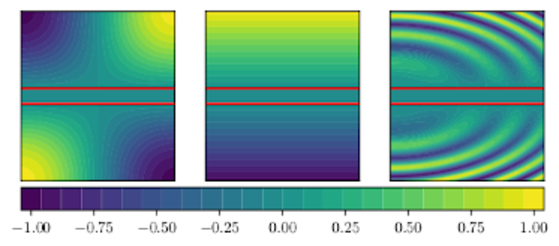
\includegraphics[scale=1.0]{Diagram_GradZeroIllustrations-Scaled.pdf}
	\caption{\label{fig:Diagram_GradZeroIllustrations} Examples illustrating how non-zero gradients of zero can arise, with the region between the red lines representing an edge $I_{jk}$, which has been thickened so one can view the function values along this edge. Despite each of the functions appearing constant along the edge $I_{jk}$, and thus constant to the measure $\lambda_{jk}$, the function is changing in the direction $n_{jk}$ as it crosses $I_{jk}$ and it's behaviour ``off the edge" is unknowable from the perspective of $\lambda_{jk}$. }
\end{figure}
Indeed, the measure $\lambda_{jk}$ is unable to deduce whether (for $x\in I_{jk}$) $u(x+hn_{jk})$ is different from $u(x)$ for $h\neq0$, given the only information it can have about $u$ are its values on $I_{jk}$.
Consequentially, $\lambda_{jk}$ can have no concept of $\pdiff{u}{n_{jk}}$ --- changing the profile of $u$ across the edge $I_{jk}$ does not change $u$ on $I_{jk}$, and consequentially the component of any ``gradient" directed along $n_{jk}$ corresponds to no change in the function $u$ from the perspective of $\lambda_{jk}$, making this component a gradient of zero.
In contrast, the measure $\lambda_{jk}$ can evaluate expressions like $u(x+he_{jk})-u(x)$ --- that is, changes in the function along $I_{jk}$ are detected by the measure $\lambda_{jk}$.
Such changes correspond to $\pdiff{u}{e_{jk}}$ being non-zero, and thus we find that tangential gradients are directed along $e_{jk}$ (and provide a ``derivative" in this direction too).
This also highlights the reason for defining the gradients of zero and tangential gradients as in section \ref{sec:BorelMeasSobSpaces} --- given a tangential gradient $\ktgrad_{\lambda_{jk}}u$, $\lambda_{jk}$ can reconstruct the function $u$ along the edge $I_{jk}$, but cannot determine what $u$ is doing across $I_{jk}$.
Ergo, every function has a gradient that is unique up to a gradient of zero, because there is no way for $\lambda_{jk}$ to determine what $u$ looks like across (and thus outside of) $I_{jk}$.

The above story is similar when considering the tangential gradient of $u$ with respect to the measure $\nu$.
Here, the ``view" of the measure is even more restricted, only being able to view the value of $u$ at the vertices, which are a set of isolated points in $\ddom$.
As such, there is no way for the measure $\nu$ to reconstruct any kind of sensible gradient --- there are no ``nearby" function values $u\bracs{v_j + h x}, x\neq 0$ to compare the value of $u\bracs{v_j}$ to.
The result is corollary \ref{cory:NuTangGradChar}, any gradient must be a gradient of zero, because as far as $\nu$ is concerned, there is no visible change in $u$ in any neighbourhood of $v_j$.
Then, given that $\dddmes$  is just the sum of the measures $\ddmes$ and $\nu$, we find that $\ktgrad_{\dddmes}u$ inherits the behaviours from $\ddmes$ and $\nu$.

\subsection{Derivation of the system \eqref{eq:SingularWaveEqnQGProblem}} \label{ssec:Scalar-QGDerivation}
We can now provide an argument for how a system of the form \eqref{eq:SingularWaveEqnQGProblem} arises from \eqref{eq:SingularScalarWaveEqn}.
Take any $\varphi\in\csmooth{\sqbracs{0,l_{jk}}}$ and let $\phi\in\psmooth{\ddom}$ be such that $\phi\circ r_{jk} = \varphi$ on $\sqbracs{0,l_{jk}}$, with $\supp\phi\cap\graph\subset I_{jk}^{\circ}$.
Recall that the change of variables $r_{jk}$ is affine (see \eqref{eq:EdgeParameterisation}), so in particular this change of variables is invertable.
Testing against such $\phi$ in \eqref{eq:SingularScalarWaveEqn-VariationalForm}, combined with the fact that $\dddmes$ is a sum of the edge measures and point masses at the vertices, and that $\tgrad_{\dddmes}u=\tgrad_{\lambda_{jk}}u$ on the edge $I_{jk}$, equation \eqref{eq:SingularScalarWaveEqn-VariationalForm} implies
\begin{align*}
	0 &= \integral{\ddom}{ \bracs{\tgrad_\ddmes u \cdot \overline{\tgrad\phi} - \omega^2 u\overline{\phi}} }{\ddmes}
	= \integral{I_{jk}}{ \bracs{\tgrad_{\lambda_{jk}}u \cdot \overline{\tgrad\phi} - \omega^2 u^{(jk)}\overline{\phi}} }{\lambda_{jk}} \\
	&= \integral{I_{jk}}{ \clbracs{ \bracs{\bracs{u^{(jk)}}' + \rmi\qm_{jk} u^{(jk)}}\bracs{\overline{\phi}' - \rmi\qm_{jk} \overline{\phi} } - \omega^2 u^{(jk)}\overline{\phi} } }{\lambda_{jk}}.
\end{align*}
Now using the change of variables $r_{jk}$ and denoting $\tilde{u}^{(jk)} = u^{(jk)} \circ r_{jk}$, we arrive at
\begin{align*}
	0 &= \int_{0}^{l_{jk}} \bracs{\bracs{\tilde{u}^{(jk)}}' + \rmi\qm_{jk} \tilde{u}^{(jk)}}\bracs{\overline{\varphi}' - \rmi\qm_{jk} \overline{\varphi} } - \omega^2 \tilde{u}^{(jk)}\overline{\varphi} \ \md y. \\
	\implies
	\int_{0}^{l_{jk}} \bracs{\tilde{u}^{(jk)}}'\overline{\varphi}' \ \md y &=
	\int_{0}^{l_{jk}} \clbracs{ \omega^2\tilde{u}^{(jk)} + 2\rmi\qm_{jk}\bracs{\tilde{u}^{(jk)}}' + \bracs{\rmi\qm_{jk}}^2\tilde{u}^{(jk)} } \overline{\varphi} \ \md y.
\end{align*}
This holds for all $\varphi\in\csmooth{\sqbracs{0,l_{jk}}}$, and thus implies that $\tilde{u}^{(jk)}$ is twice (weakly) differentiable along $\sqbracs{0,l_{jk}}$.
Furthermore, we then obtain the (strong) equation
\begin{align*}
	-\bracs{\diff{}{y} + \rmi\qm_{jk}}^2 \tilde{u}^{(jk)} &= \omega^2 \tilde{u}^{(jk)}, \quad y\in\sqbracs{0,l_{jk}}.
\end{align*}

Now we turn our attention to the derivation of the vertex conditions.
Fix a vertex $v_j\in \vertSet$, and consider functions $\phi\in\psmooth{\ddom}$ with $\supp\phi\cap\graph\subset \mathcal{J}(v_j)\setminus\clbracs{v_j}$ (that is, smooth functions that are only non-zero on $\graph$ close to the vertex $v_j$).
Using the change of variables $r_{jk}$ on each edge and writing $\tilde{u}^{(jk)} = u^{(jk)} \circ r_{jk}$, $\varphi_{jk} = \phi\circ r_{jk}$ for each $k\con j$, we can work from \eqref{eq:SingularScalarWaveEqn-VariationalForm} to obtain
\begin{align*}
	0 &= \sum_{k: \ k\con j} \integral{I_{jk}}{ \bracs{ \tgrad_\ddmes u \cdot \overline{\tgrad\phi} - \omega^2 u\overline{\phi} } }{\lambda_{jk}} 
	+ \integral{\ddom}{ \bracs{ \tgrad_{\dddmes}u\cdot\overline{\tgrad_{\dddmes}\phi}-\omega^2 u\overline{\phi} } }{\massMes} \\
	&= \sum_{k: \ k\con j} \int_{0}^{l_{jk}} \clbracs{ \bracs{\bracs{\tilde{u}^{(jk)}}' + \rmi\qm_{jk} \tilde{u}^{(jk)}}\bracs{\overline{\varphi}_{jk}' - \rmi\qm_{jk} \overline{\varphi}_{jk} } - \omega^2 \tilde{u}^{(jk)}\overline{\varphi}_{jk} } \ \md y \\
	&\qquad + \alpha_j\left.\bracs{ \tgrad_{\dddmes}u\cdot\overline{\tgrad_{\dddmes}\phi}-\omega^2 u\overline{\phi} }\right\vert_{v_j} \\
	&= \sum_{k: \ k\con j} \int_{0}^{l_{jk}} \clbracs{ \bracs{\bracs{\tilde{u}^{(jk)}}' + \rmi\qm_{jk} \tilde{u}^{(jk)}}\bracs{\overline{\varphi}_{jk}' - \rmi\qm_{jk} \overline{\varphi}_{jk} } - \omega^2 \tilde{u}^{(jk)}\overline{\varphi}_{jk} } \ \md y
	 - \alpha_j \omega^2 u\bracs{v_j}\overline{\phi}\bracs{v_j}.
\end{align*}
Here we have used the fact that $\tgrad_{\dddmes}u\bracs{v_j}=0$ (see section \ref{sec:3DGradSobSpaces}).
Given that (from our considerations along the edges) $u$ is twice differentiable on each $I_{jk}$, and $\phi$ is zero at every vertex except $v_j$, it follows that
\begin{align*}
	\alpha_j\omega^2 u\bracs{v_j}\overline{\phi}\bracs{v_j} 
	&= - \sum_{k: \ k\con j} \int_{0}^{l_{jk}} \bracs{ \bracs{\diff{}{x} + \rmi\qm_{jk}}^2 \tilde{u}^{(jk)} +\omega^2 \tilde{u}^{(jk)} }\overline{\varphi}_{jk} \ \md y \\
	&\qquad + \sum_{k: \ k\con j}\overline{\varphi}_{jk}\bracs{v_j}\bracs{\pdiff{}{n} + \rmi\qm_{jk}}\tilde{u}^{(jk)}\bracs{v_j} \\
	&= \overline{\phi}\bracs{v_j}\sum_{k: \ k\con j}\bracs{\pdiff{}{n} + \rmi\qm_{jk}}\tilde{u}^{(jk)}\bracs{v_j}. \labelthis\label{eq:DerivationVertexConditionWeak}
\end{align*}
Given that \eqref{eq:DerivationVertexConditionWeak} holds for every smooth $\varphi$, and that $\varphi_{jk}\bracs{v_j}=\phi\bracs{v_j}$, we arrive at the condition
\begin{align*}
	\alpha_j\omega^2 u\bracs{v_j} &= \sum_{j\con k}\bracs{\pdiff{}{n} + \rmi\qm_{jk}}\tilde{u}^{(jk)}\bracs{v_j}.
\end{align*}

Repeating the argument for each $v_j\in \vertSet$ then provides us with a condition of this form at each vertex.
One should note the presence of $\omega^2$ in this equation, so this is not a Kirchoff condition on the derivatives of the edge functions $u^{(jk)}$, and indicates that the problem we have arrived at is defined through an operator acting in an extended space, as mentioned in section \ref{ssec:DiffOpsOnGraphs}.
The result of theorem \ref{thm:dddmesTangGradImplication} tells us that functions $u\in\gradSobQM{\ddom}{\dddmes}$ are also continuous at each vertex $v_j$, and thus the following problem (precisely \eqref{eq:SingularWaveEqnQGProblem}) has been derived:
\begin{subequations}
	\begin{align*}
		-\bracs{\diff{}{y} + \rmi\qm_{jk}}^2 u^{(jk)} &= \omega^2 u^{(jk)}, \quad &y\in\sqbracs{0,l_{jk}}, \ \forall I_{jk}\in\edgeSet, \tag{\eqref{eq:SingularWaveEqnQGProblem-1} restated} \\
		u \text{ is continuous at } & v_j, \quad &\forall v_j\in\vertSet,  \tag{\eqref{eq:SingularWaveEqnQGProblem-2} restated} \\
		\sum_{j\con k}\bracs{\pdiff{}{n} + \rmi\qm_{jk}}u^{(jk)}\bracs{v_j} &= \omega^2\alpha_j u\bracs{v_j}, \quad &\forall v_j\in\vertSet, \tag{\eqref{eq:SingularWaveEqnQGProblem-3} restated}
	\end{align*}
\end{subequations}
where we henceforth drop the overhead tilde notation and simply write $u^{(jk)}$ for brevity (appealing to the obvious association between $u^{(jk)}$ and $\tilde{u}^{(jk)}$).
As will be made clear in the discussion that follows, the quantum graph problem \eqref{eq:SingularWaveEqnQGProblem} is much easier to handle (than \eqref{eq:SingularScalarWaveEqn}) analytically and numerically thanks to the utility of the $M$-matrix.

Now that we have obtained the system \eqref{eq:SingularWaveEqnQGProblem}, we can affirm our interpretation of the coupling constants $\alpha_j$ as the (limit of the) ratio of vertex volume $V_{\mathrm{vertex}}$ to edge volume $V_{\mathrm{edge}}$ that was described in section \ref{ssec:Intro-ThinStructures}.
As can clearly be seen from \eqref{eq:SingularWaveEqnQGProblem-3}, when $\alpha_j$ is non-zero and finite, we obtain Wentzell conditions between the incoming derivatives to the vertex $v_j$.
This is precisely the boundary condition we would obtain in the zero-thickness limit for the (Neumann) Laplacian on a thickened graph, provided the ratio $\frac{V_{\mathrm{vertex}}}{V_{\mathrm{edge}}}\rightarrow\alpha_j$ as the thickness of the structure tended to zero.
Moreover, notice that if $\alpha_j=0$ in \eqref{eq:SingularWaveEqnQGProblem-3}, we obtain an exact Kirchoff condition at the vertex $v_j$, along with continuity of the incoming edge functions --- precisely the case when $V_{\mathrm{vertex}}\ll V_{\mathrm{edge}}$.
Finally, if one divides through by $\alpha_j$ in \eqref{eq:SingularWaveEqnQGProblem-3} and takes a formal limit as $\alpha_j\rightarrow\infty$, the resulting system imposes homogeneous Dirichlet boundary conditions on the solution $u$ at $v_j$ --- corresponding to the conditions obtained in the limiting case $V_{\mathrm{vertex}}\gg V_{\mathrm{edge}}$.
We can also predict the resulting problems of thickened graphs that possess a mixture of vertex and edge volumes; that is when a thickened graph $\mathcal{G}_{\delta}$ of $\graph$ is such that $V_{\mathrm{edge}}\bracs{\delta}$ is the same for every (thickened) edge, yet the scaling of the volume of the thickened vertices $V_{v_j}\bracs{\delta}, v_j\in\vertSet$ with $\delta$ changes between vertices.
Letting $\alpha_j = \lim_{\delta\rightarrow0}\frac{V_{v_j}}{V_{\mathrm{edge}}}$ (where we formally allow $\alpha_j=\infty$) for each $v_j$, our consideration of singular measures and the variational problem \eqref{eq:SingularScalarWaveEqn} predicts that the resulting system will be realisable as the following quantum graph problem:
\begin{subequations}
	\begin{align*}
		-\bracs{\diff{}{y} + \rmi\qm_{jk}}^2 u^{(jk)} &= \omega^2 u^{(jk)}, \quad & y\in\sqbracs{0,l_{jk}}, \ \forall I_{jk}\in\edgeSet, \\
		u \text{ is continuous at } & v_j, \quad &\forall v_j\in\vertSet, \\
		\sum_{j\con k}\bracs{\pdiff{}{n} + \rmi\qm_{jk}}u^{(jk)}\bracs{v_j} &= \omega^2\alpha_j u\bracs{v_j}, \quad &\forall v_j\in\vertSet, \ \alpha_j\in\bracs{0,\infty}, \\
		\sum_{j\con k}\bracs{\pdiff{}{n} + \rmi\qm_{jk}}u^{(jk)}\bracs{v_j} &= 0, \quad &\forall v_j\in\vertSet, \ \alpha_j = 0, \\
		u\bracs{v_j} &= 0, \quad &\forall v_j\in\vertSet, \ \alpha_j = \infty.
	\end{align*}
\end{subequations}
We also remark that, for a graph with $\alpha_j<\infty$ for every $v_j$, our approach via the $M$-matrix (section \ref{sec:ScalarDiscussion}) for determining the spectrum of the above problem can be employed.

\subsection{The relation between $\tgradSob{\ddom}{\dddmes}$ and extended spaces} \label{ssec:ExtendedSpaces}
As we have already discussed, the problem \eqref{eq:SingularWaveEqnQGProblem} coincides with the problems that arise in the zero-thickness limit of thin-structures.
Indeed, the system \eqref{eq:SingularWaveEqnQGProblem} corresponds to the operator $\mathcal{A}_{\mathrm{ext}}$ that acts in the \emph{extended space}
\begin{align*}
	\dom\mathcal{A}_{\mathrm{ext}} 
	&= \clbracs{ (u, \beta) \setVert u\in H^2\bracs{\graph}, \ u \text{ is continuous at each } v_j\in\vertSet, \ \beta_j=\alpha_j u(v_j) } \\
	& \subset L^2\bracs{\graph}\oplus\complex^{\abs{\vertSet}}.
\end{align*}
The element $\bracs{u,\beta}$ is a $\abs{\edgeSet}+\abs{\vertSet}$ ``vector" (more precisely, tuple) consisting of the edge functions $u^{(jk)}$, followed by the (scaled) vertex values $\beta_j$, which we shall write as
\begin{align*}
	\begin{pmatrix} u \\ \beta \end{pmatrix}
	&= \begin{pmatrix} \clbracs{u^{(jk)}}_{I_{jk}\in\edgeSet} \\ \clbracs{\beta_j}_{v_j\in\vertSet} \end{pmatrix}.
\end{align*}
The action of $\mathcal{A}_{\mathrm{ext}}$ defined as
\begin{align*}
	\mathcal{A}_{\mathrm{ext}} \begin{pmatrix} u \\ \beta \end{pmatrix}
	&= 
	\begin{pmatrix}
		\clbracs{-\bracs{\diff{}{y}+\rmi\qm_{jk}}^2 u^{(jk)}}_{I_{jk}\in\edgeSet} \\ 
		\clbracs{\sum_{j\con k}\bracs{ \pdiff{}{n} + \rmi\qm_{jk} }u^{(jk)}(v_j)}_{v_j\in\vertSet}
	\end{pmatrix},
\end{align*}
the space $L^2\bracs{\graph}\oplus\complex^{\abs{\vertSet}}$ is the extended space, and $\mathcal{A}_{\mathrm{ext}}$ the Strauss extension for the problem \eqref{eq:SingularWaveEqnQGProblem}.

It is clear that the operators $\mathcal{A}_{\mathrm{ext}}$ and $-\laplacian_{\dddmes}^{\qm}$ possess the same spectrum and eigenfunctions, by virtue of theorem \ref{thm:CharOfSobSpaces}.
Now let $f\in L^2\bracs{\graph}\oplus\complex^{\abs{\vertSet}} \cong \ltwo{\ddom}{\dddmes}$.
Setting aside questions of solubility for the time being, a solution to the problem $\mathcal{A}_{\mathrm{ext}}u=f$ is also guaranteed to provide a solution to $-\laplacian_{\qm}^{\dddmes}u=f$ and vice-versa through this theorem.
The converse also assured upon realising the problem $-\laplacian_{\qm}^{\dddmes}u=f$ can be written in the form \eqref{eq:SingularWaveEqnQGProblem}\footnote{The fact that $f\in\ltwo{\ddom}{\dddmes}$ is important here, as it provides enough regularity for $u$ to be an element of $H^2\bracs{\graph}$.}, except replacing $\omega^2 u$ with $f$ in \eqref{eq:SingularWaveEqnQGProblem-1} and $\omega^2\alpha_j u(v_j)$ with $\alpha_j f(v_j)$ in \eqref{eq:SingularWaveEqnQGProblem-3}.
Our approach via singular measures has resulted in the immediate construction of the extended space \emph{and corresponding operator} one obtains in the zero-thickness limit of thin-structure problems.
Within the context of the acoustic approximation we already knew what these limits where, however our original formulation provides a method of defining this limiting problem by appealing to the geometry.
This also presents an opportunity we look to investigate going forward; the non-classical Sobolev spaces and variational problems provide us with a method of defining (up to isomorphism) the spaces and problems that may correspond to the --- presently unknown --- ``limits" of other thin-structure problems.

% Discussion, use of the M-matrix and solving methods
\section{General formula for the $M$-matrix of a finite period graph} \label{sec:ScalarDiscussion}
Having obtained the quantum graph problem \eqref{eq:SingularWaveEqnQGProblem}, we turn our attention to determining the eigenvalues $z := \omega^2$.
The advantage of \eqref{eq:SingularWaveEqnQGProblem} over working directly with \eqref{eq:SingularScalarWaveEqnWholeSpace} is that we can now use the $M$-matrix (introduced in section \ref{ssec:MMatrix}) as a tool in our analysis.
In this section we contextualise the theory introduced in section \ref{sec:QuantumGraphs}, and in particular section \ref{ssec:MMatrix}, showing how it is employed for studying the spectrum of \eqref{eq:SingularScalarWaveEqnWholeSpace}.
In doing so, we provide a general formula for the $M$-matrix of a finite period graph on which \eqref{eq:SingularWaveEqnQGProblem} is posed.
We will follow up on this in section \ref{sec:Examples}, where we provide some explicit examples of quantum graph problems that can be solved by employing the $M$-matrix in the manner discussed below.

\subsection{General formula for the $M$-matrix} \label{ssec:MMatrixResult}
One of the foremost advantages of the $M$-matrix is that we can explicitly (and analytically) compute its entries for any (finite period) metric graph $\graph$ on which the system \eqref{eq:SingularWaveEqnQGProblem} is posed.
We also break from assumption \ref{ass:MeasTheoryProblemSetup}, and allow for the period graph to include looping edges (edges whose endpoints correspond to same vertex), since such loops do not effect the (procedure in the) proof of the result.
The inclusion of looping edges is mostly for completeness, since when we come to use the $M$-matrix to determine the eigenvalues of \eqref{eq:SingularWaveEqnQGProblem}, we will want to introduce ``artificial vertices" (section \ref{ssec:ArtificialVertices}) to break these loops.
The following proposition provides the entries of the $M$-matrix.
\begin{prop}[$M$-matrix entries] \label{prop:M-MatrixEntries}
	Let $\graph=\bracs{\vertSet,\edgeSet}$ be an embedded graph on which the problem \eqref{eq:SingularWaveEqnQGProblem} is posed.
	Suppose that $\dmap u = e_k$ where $e_k$ is the $k$\textsuperscript{th} canonical unit vector in $\complex^{\abs{\vertSet}}$.
	Then the $j$\textsuperscript{th} entry of $\nmap u$, and hence the $jk$\textsuperscript{th} entry in the $M$-matrix, is given by
	\begin{align*}
		\bracs{\nmap u}_j &= 
		\begin{cases}
			0,	
			& j \not\con k, \\[5pt]
			\sum_{j\conLeft k} \omega \e^{\rmi\qm_{jk}l_{jk}} \csc\bracs{l_{jk}\omega} 
			+ \sum_{j\conRight k} \omega \e^{-\rmi\qm_{kj}l_{kj}} \csc\bracs{l_{kj}\omega},
			& j\neq k, \ j\con k, \\[5pt]
			- \sum_{\substack{j\con l \\ j\neq l}} \omega\cot\bracs{l_{jl}\omega}
			- 2\omega\sum_{j\conLeft j} \clbracs{ \cot\bracs{l_{jj}\omega} - \cos\bracs{\qm_{jj}l_{jj}}\csc\bracs{l_{jj}\omega} },
			& j=k.
		\end{cases}
	\end{align*}
\end{prop}
Note the choice of $j\conLeft j$ in the contributions from loops is simply a convention, $j\conRight j$ is equivalent here.
Also recall the convention for summing over $j\con k$:
\begin{align*}
	\sum_{j\con k} \omega\cot\bracs{l_{jk}\omega} &= \sum_{j\conLeft k} \omega\cot\bracs{l_{jk}\omega}	+ \sum_{j\conRight k} \omega\cot\bracs{l_{kj}\omega}
\end{align*}
\begin{proof}
	The proof below is an explicit computation, similar to that in \cite{ershova2014isospectrality} with adjustments for the dependence on $\qm$.
	
	We first write the general form of the edge solution $u^{(jk)}$ from \eqref{eq:SingularWaveEqnQGProblem-1}:
	\begin{align} \label{eq:EdgeEqnGeneralSolution}
		u^{(jk)} &= \e^{-\rmi\qm_{jk}t}\bracs{ C_{+}^{(jk)}\e^{-\rmi\omega x} + C_{-}^{(jk)}\e^{\rmi\omega x} },
		\quad C_{+}^{(jk)}, C_{-}^{(jk)}\in\complex.
	\end{align}
	Since the $M$-matrix maps $\complex^{\abs{\vertSet}}$ to $\complex^{\abs{\vertSet}}$, it is sufficient to determine its action on the canonical basis of $\complex^{\abs{\vertSet}}$.
	So for each fixed $k\in\clbracs{1,...,\abs{\vertSet}}$ we set $\dmap u = e_k$.
	This provides us with sufficient Dirichlet data to solve \eqref{eq:SingularWaveEqnQGProblem-1} on each edge and eliminate the constants $C_{+}^{(jk)}$, $C_{-}^{(jk)}$ in \eqref{eq:EdgeEqnGeneralSolution}, obtaining
	\begin{align*}
		j\not\con k &\implies
		\begin{cases}
			u_{jk}(x) = 0, \\
			u_{kj}(x) = 0,
		\end{cases} \\
		j\neq k, \ j\con k &\implies
		\begin{cases}
			u_{jk}(x) = \e^{-\rmi\qm_{jk}\bracs{x-l_{jk}}}\csc\bracs{\omega l_{jk}}\sin\bracs{\omega x}, \\
			u_{kj}(x) = \e^{-\rmi\qm_{kj}x}\csc\bracs{\omega l_{kj}}\sin\bracs{\omega \bracs{l_{kj}-x}},
		\end{cases} \\
		j = k &\implies 
		\begin{cases}
			u_{jj}(t) = \e^{-\rmi\qm_{jj}x} \bracs{ \e^{-\rmi\omega x} + \sqbracs{\e^{\rmi\qm_{jj}l_{jj}}-\e^{-\rmi\omega l_{jj}}}\csc\bracs{\omega l_{jj}}\sin\bracs{\omega x}  },
		\end{cases}
	\end{align*}
	This in turn enables us to explicitly differentiate the expressions for $u_{jk}$, and read off the values of $\bracs{\pdiff{}{n}+\rmi\qm_{jk}}u_{jk}$ at the vertices.
	In the case $j\not\con k$, we obviously get zero contribution from the edges $I_{jk}$ and $I_{kj}$.
	The case $j\neq k, \ j\con k$, yields the following contributions from the edges $I_{jk}$ and $I_{kj}$:
	\begin{align*}
		\bracs{\pdiff{}{n}+\rmi\qm_{jk}}u^{(jk)}\bracs{v_j} = -\omega \e^{\rmi\qm_{jk}l_{jk}}\csc\bracs{\omega l_{jk}}, 
		&\qquad \bracs{\pdiff{}{n}+\rmi\qm_{jk}}u^{(jk)}\bracs{v_k} = \omega\cot\bracs{\omega l_{jk}}, \\
		\bracs{\pdiff{}{n}+\rmi\qm_{kj}}u^{(kj)}\bracs{v_j} = -\omega \e^{-\rmi\qm_{kj}l_{kj}}\csc\bracs{\omega l_{kj}}, 
		&\qquad \bracs{\pdiff{}{n}+\rmi\qm_{kj}}u^{(kj)}\bracs{v_k} = \omega\cot\bracs{\omega l_{kj}}.
	\end{align*}
	Finally, when considering the case $j=k$, the contribution to $\bracs{\nmap u}_j$ from loops $I_{jj}$ in the graph also requires us to compute
	\begin{align*}
		-\lim_{x\rightarrow0}\bracs{\bracs{u^{(jj)}}'+i\qm_{jj}u^{(jj)}}(x) + \lim_{x\rightarrow l_{jj}} & \bracs{\bracs{u^{(jj)}}'+i\qm_{jj}u^{(jj)}}(x) \\
		&\qquad = 2\omega\bigl( \cot\bracs{\omega l_{jj}} - \cos\bracs{\qm_{jj}l_{jj}}\csc\bracs{\omega l_{jj}} \bigr).	
	\end{align*}
	We then use the formula
	\begin{align*}
		\bracs{\nmap u}_j &= -\sum_{j\con l} \bracs{\pdiff{}{n}+\rmi\qm_{jl}}u^{(jl)}\bracs{v_j},
	\end{align*}
	which yields the desired result.
\end{proof}

Proposition \ref{prop:M-MatrixEntries} also explicitly demonstrates that the $M$-matrix (in the context of \eqref{eq:SingularWaveEqnQGProblem}) is parametrised by $\qm$, and so we shall denote it by $M_{\qm}$ henceforth.
The dependence of $M_\qm$ on $\qm$ is due to our decision to specify our singular structure (comprising the domain in which \eqref{eq:SingularScalarWaveEqnWholeSpace} was posed) as an embedded, periodic metric graph and then apply the Gelfand transform (see section \ref{ssec:MMatrix}).
In the following section, we continue our analysis of the $M$-matrix and outline how it can be used to recover the eigenvalues $z=\omega^2$ of \eqref{eq:SingularWaveEqnQGProblem}, and thus \eqref{eq:SingularScalarWaveEqnWholeSpace}.

\subsection{Consequences of Proposition \ref{prop:M-MatrixEntries}} \label{ssec:MMatrixConsequences}
Whilst proposition \ref{prop:M-MatrixEntries} provides an explicit form for the entries of the $M$-matrix,  it is not the most convenient when looking for a method for determining the spectrum of \eqref{eq:SingularWaveEqnQGProblem}.
Proposition \ref{prop:M-MatrixEntries} shows that $M_\qm$ is meromorphic, and thus has the following decomposition:
\begin{cory} \label{cory:M-MatrixEntriesNoPoles}
	Let $G^{(1)}_\qm\bracs{\omega}$ have entries defined by
	\begin{align*}
		\bracs{G^{(1)}_\qm}_{jk} &= 
		\begin{cases}
			\!\begin{aligned}
				&0,
			\end{aligned}			
			& j \not\con k, \\
			\!\begin{aligned}
				&\sum_{j\conLeft k} \bracs{ \e^{\rmi\qm_{jk}l_{jk}} \prod_{v_l\in\vertSet}\prod_{\substack{ l\conLeft m \\ \bracs{l,m} \neq \bracs{j,k} }}\sin\bracs{l_{lm}\omega} }
				\\ &\quad + \sum_{j\conRight k} \bracs{ \e^{-\rmi\qm_{kj}l_{kj}} \prod_{v_l\in\vertSet}\prod_{\substack{l\conLeft m \\ \bracs{l,m} \neq \bracs{k,j} }}\sin\bracs{l_{lm}\omega} },
			\end{aligned}
			& j\neq k, \ j\con k, \\
			\!\begin{aligned}
				&- \sum_{\substack{j\con l \\ j\neq l}} \bracs{ \cos\bracs{l_{jl}\omega}\prod_{v_m\in\vertSet}\prod_{\substack{ m\conLeft n \\ \bracs{m,n}\neq\bracs{j,l} }}\sin\bracs{l_{mn}\omega} }
				\\ &\quad - 2\sum_{j\conLeft j} \bracs{ \sqbracs{ \prod_{v_l\in\vertSet}\prod_{\substack{l\conLeft m \\ \bracs{l,m}\neq\bracs{j,j} }}\sin\bracs{l_{lm}\omega} }\bigl[ \cos\bracs{l_{jj}\omega} - \cos\bracs{\qm_{jj}l_{jj}} \bigr] },
			\end{aligned}
			& j=k,
		\end{cases}
	\end{align*}
	and set
	\begin{align*}
		G^{(2)}\bracs{\omega} &= \prod_{v_j\in\vertSet} \prod_{j\conLeft k}\sin\bracs{l_{jk}\omega}.
	\end{align*}
	Further define
	\begin{align*}
		H^{(1)}_{\qm}(z) &:= 
		\begin{cases} 
			\omega G_\qm^{(1)}(\omega), & \abs{\edgeSet} \text{ is even}, \\
			G_\qm^{(1)}(\omega), & \abs{\edgeSet} \text{ is odd},
		\end{cases} \\
		H^{(2)}(z) &:=
		\begin{cases}
			G^{(2)}(\omega), & \abs{\edgeSet} \text{ is even}, \\
			\omega^{-1} G^{(2)}(\omega), & \abs{\edgeSet} \text{ is odd}.
		\end{cases}
	\end{align*}
	Then the functions $H^{(1)}_{\qm}(z)$ and $H^{(2)}(z)$ are analytic in $z:=\omega^2$ and we have
	\begin{align*}
		M_\qm\bracs{z} &= \bracs{ H^{(2)}\bracs{z} }^{-1} H^{(1)}_\qm\bracs{z}.
	\end{align*}
\end{cory}
The product notation should be understood analogously to the summation notation over $j\con k$ introduced in section \ref{sec:QuantumGraphs}.
The zeros of $H^{(2)}$ exactly coincide with the poles of $M_\qm$, both $H^{(1)}_\qm$ and $H^{(2)}$ are analytic, and the matrix $H^{(1)}_\qm$ even has its entry at position $jk$ bounded (uniformly in $\omega$) by the number of (direct) connections between $v_j$ and $v_k$.

Recall that (section \ref{ssec:MMatrix}) we need to determine those $z$ for which the matrix $M_\qm(z)-B(z)$ has at least one zero eigenvalue, where we have $B(z) = -z\alpha$.
Note the dependence of $B$ on $z$ --- this was raised in section \ref{ssec:DiffOpsOnGraphs}.
Now let $\beta_j\bracs{z}, j\in\clbracs{1,...,\abs{\vertSet}}$ denote the eigenvalue branches of the matrix $M_\qm(z)-B(z)$.
Also set $\mathfrak{M}_\qm(z) = H^{(1)}_\qm(z) - H^{(2)}(z)B(z)$, and let $\widetilde{\beta}_j\bracs{z}, j\in\clbracs{1,...,\abs{\vertSet}}$ denote the eigenvalue branches of $\mathfrak{M}_\qm$.
The matrix $\mathfrak{M}_\qm$ is analytic, and so has at least one zero eigenvalue at those $z$ for which there exists a $w\in\complex^{\abs{\vertSet}}\setminus\clbracs{0}$ such that
\begin{align} \label{eq:QGGenEvalSolveNoPoles}
	\mathfrak{M}_\qm\bracs{z}w = 0.
\end{align}
We could also chose to determine these $z$ via solution to 
\begin{align} \label{eq:QGDetSolveCondition}
	\det\mathfrak{M}_\qm\bracs{z} &= 0,
\end{align}
the merits of each approach (via \eqref{eq:QGGenEvalSolveNoPoles} or \eqref{eq:QGDetSolveCondition}) we will discuss in section \ref{ssec:ApproachConsiderations}.
If $z_0$ solves \eqref{eq:QGGenEvalSolveNoPoles} (or equivalently \eqref{eq:QGDetSolveCondition}), then $M_{\qm}\bracs{z_0}-B\bracs{z_0}$ has a zero eigenvalue when
\begin{align} \label{eq:EigenvalueBranchLimit}
	\lim_{z\rightarrow z_0} \beta_j\bracs{z} = \lim_{z\rightarrow z_0} \bracs{ H^{(2)}\bracs{z} }^{-1} \widetilde{\beta}_j\bracs{z} = 0
\end{align}
for at least one $j$ with $\widetilde{\beta}_j\bracs{z_0}=0$.
Checking the limit in \eqref{eq:EigenvalueBranchLimit} is not necessary for all solutions $z_0$ to \eqref{eq:QGDetSolveCondition}; provided that $H^{(2)}\bracs{z_0}\neq 0$, which by corollary \ref{cory:M-MatrixEntriesNoPoles} occurs when
\begin{align*}
	z_0 \neq \bracs{ \frac{n\pi}{l_{jk}} }^2, \quad j\conLeft k, \ n\in\naturals_{0},
\end{align*}
the limit in \eqref{eq:EigenvalueBranchLimit} is clearly zero, and so $z_0$ belongs to the spectrum of \eqref{eq:SingularWaveEqnQGProblem}.
As we will discuss in section \ref{ssec:ApproachConsiderations}, checking the limit \eqref{eq:EigenvalueBranchLimit} may not be necessary at all, given known results about the spectra of periodic quantum graph problems.
Considerations concerning which of the two equations (\eqref{eq:QGGenEvalSolveNoPoles} or \eqref{eq:QGDetSolveCondition}) should be used for determining the spectrum $\sigma_\qm$ are also discussed in section \ref{ssec:ApproachConsiderations}.
In any event, \eqref{eq:SingularScalarWaveEqnWholeSpace} has now been reduced to a more accessible (family of) matrix-eigenvalue problems for $\mathfrak{M}_\qm$.

\subsection{Artificial Vertices and Splitting Edges} \label{ssec:ArtificialVertices}
As noted in section section \ref{ssec:MMatrix}, it is required that the underlying graph $\graph$ contains no looping edges and has all edge-lengths pairwise irrationally-related.
Failure to ensure that this condition is met may result in the ``loss" of certain eigenvalues when using the $M$-matrix to determine the spectrum of \eqref{eq:SingularWaveEqnQGProblem} --- these are highlighted explicitly in section \ref{ssec:Example1DLoop}.
Of course, the graphs motivated by physical applications generally do not adhere to these restrictions, so it is necessary to introduce ``artificial" or ``dummy" vertices.
These artificial vertices ``split" edges of the original graph, removing any loops and ensuring all (new) edges have irrationally-related lengths.

Introducing an artificial vertex to split an edge is as intuitive as it sounds --- suppose $\graph=\bracs{\vertSet, \edgeSet}$ and one wishes to ``split" the edge $I_{jk}$ (where it may be the case that $j=k$).
Place a vertex $v_l$ at some point along the edge $I_{jk}$, and replace $I_{jk}$ with the edges $I_{jl}$ and $I_{lk}$, to obtain a new graph $\graph^*$.
The total length of the edges must be preserved, so $\abs{I_{jk}} = \abs{I_{jl}}+\abs{I_{lk}}$, but the lengths of the new edges should be chosen in accordance with the requirements above in mind.
Furthermore, a zero coupling constant should be placed at the artificial vertex $v_l$ --- this ensures matching of the solution $u$ and its derivative at the artificial vertex, as would have been the case along the original edge if it had not been split.
The quasi-momentum parameters should also satisfy $\qm_{jl}=\qm_{lk}=\qm_{jk}$ (although this is a by-product of having straight edges, see assumption \ref{ass:MeasTheoryProblemSetup}).
This ensures (via \eqref{eq:SingularWaveEqnQGProblem-2} and \eqref{eq:SingularWaveEqnQGProblem-3}) that any eigenvalues $\omega^2$ of \eqref{eq:SingularWaveEqnQGProblem} on $\graph^*$ are also eigenvalues of \eqref{eq:SingularWaveEqnQGProblem} on $\graph$, with the eigenfunction $u^{(jk)}$ being related to $u^{(jl)}$ and $u^{(lk)}$ in the obvious manner.
This process can be iterated, splitting edges iteratively to remove rational-relations between edge lengths, and any loops themselves.
Doing so means that any graph representing a singular-structure can now be treated in the manner described in section \ref{ssec:MMatrixConsequences}.

\subsection{Considerations for the Approach to Solving \eqref{eq:QGGenEvalSolveNoPoles} or \eqref{eq:QGDetSolveCondition}} \label{ssec:ApproachConsiderations}
In this section we briefly discuss some considerations for recovering the spectrum of \eqref{eq:SingularScalarWaveEqnWholeSpace} (which we denote by $\sigma$), and the merits of determining the spectrum of \eqref{eq:SingularWaveEqnQGProblem} (denoted $\sigma_\qm$) via \eqref{eq:QGGenEvalSolveNoPoles} or \eqref{eq:QGDetSolveCondition}.
Recall that our use of the Gelfand transform informs us that $\sigma = \bigcup_{\qm}\sigma_{\qm}$.
We also take as a baseline that one has to hand an appropriate numerical scheme for handling the generalised eigenvalue problem \eqref{eq:QGGenEvalSolveNoPoles} (a good introduction to which can be found in \cite{guttel2017nonlinear}), and so do not delve into the details of how such an algorithm would operate.
It is however worth mentioning that $\mathfrak{M}_\qm$ is Hermitian, from which most numerical schemes benefit.

There are also several known results concerning the spectra of (periodic) quantum graphs, and here we highlight those most relevant to our context. 
A detailed discussion of the spectral structure of (periodic) quantum graphs, including statements (and proofs) of the results cited here, can be found in \cite[Chapter 4]{berkolaiko2013introduction}.
Foremost, it is known that there exist real numbers $a_j, b_j, j\in\naturals$ such that $\sigma = \bigcup_{j\in\naturals}\sqbracs{a_j,b_j}$ --- $\sigma$ is said to have a \emph{band-gap structure} or \emph{representation} \cite[Chapter 4.3]{berkolaiko2013introduction} if this is the case.
The \emph{spectral bands} are the intervals $I_j=\sqbracs{a_j,b_j}, \ j\in\naturals$, with the regions between $b_j$ and $a_{j+1}$ being referred to as \emph{spectral gaps}, where there are no eigenvalues.
For this reason the points $a_j$ and $b_j$ sometimes referred to as the \emph{spectral edges}, and in general $a_j\rightarrow\infty$ as $j\rightarrow\infty$.
Knowing that $\sigma$ has a band-gap representation is particularly useful when attempting to use either \eqref{eq:QGGenEvalSolveNoPoles} or \eqref{eq:QGDetSolveCondition} to determine it, which we will touch on shortly.
Other notable results are that $\sigma$ has no singular continuous part (\cite[Chapter 4.4]{berkolaiko2013introduction}) but may have non-empty pure-point part (\cite[Chapter 4.5]{berkolaiko2013introduction}) --- a non-empty pure-point spectrum implies the existence of a compactly supported eigenfunction for the graphs considered in this work.

Using corollary \ref{cory:M-MatrixEntriesNoPoles}, the following proposition can be proved.
\begin{prop} \label{prop:MMatrixDetForm}
	Given a graph $\graph = \bracs{\vertSet, \edgeSet}$, with the lengths of the edges of $\graph$ pairwise-irrationally related, there exists a function $F\bracs{\qm,\omega}$ such that
	\begin{align} \label{eq:MMatrixDetForm}
		\det\mathfrak{M}_\qm\bracs{\omega^2} = \bracs{ \omega H^{(2)}\bracs{\omega^2} }^{\abs{\vertSet}-2} F\bracs{\qm,\omega}.
	\end{align}
	Furthermore, $F\bracs{\qm,\omega}$ is analytic in both its arguments.
\end{prop}
The proof of this result can be found in section \ref{sec:ProofOfProp}, but essentially involves counting the number of times a given factor can appear in the expression for the determinant.
The prefactor $\bracs{ \omega H^{(2)}\bracs{\omega^2} }^{\abs{\vertSet}-2}$ informs us that checking \eqref{eq:EigenvalueBranchLimit} will be necessary for all the roots of $H^{(2)}$.
The set $F_0 := \clbracs{\omega \setVert \exists\qm \text{ s.t. }F\bracs{\qm, \omega}=0}$ then determines the remainder of $\sigma$ --- so in particular, the function $F$ determines the ``width" of the spectral bands, or the vast majority of the spectrum.
Finding $\sigma$ (up to checking roots of $H^{(2)}$) now becomes a question of obtaining $F_0$ efficiently.
One can always take the ``brute-force" approach: compute $F_0^{\qm} := \clbracs{\omega \setVert F\bracs{\qm, \omega}=0}$ for each $\qm$ (or for each $\qm$ in a suitable mesh if working numerically), and then take the union over $\qm$ to obtain $F_0$.
This is computationally expensive (both numerically and analytically) and ``brute force" should only be a last resort, so we highlight some alternatives.

If we can write $F\bracs{\qm,\omega} = F_1\bracs{\qm} - F_2\bracs{\omega}$ for continuous $F_1$ and $F_2$, then \eqref{eq:QGDetSolveCondition} implies $F_0$ can be found simply by examining
\begin{align*}
	\min_{\qm}\clbracs{F_1(\qm)} \leq F_2\bracs{\omega} \leq \max_{\qm}\clbracs{F_1(\qm)},
\end{align*} 
although such a separation of $F$ will not generally be possible, and this also relies finding an analytic expression for $\det\mathfrak{M}_\qm$.
One can always ask the more general question of whether, given the knowledge that $\sigma$ has a band-gap structure, an alternative to finding all $\omega\in F_0$ is to only compute the spectral edges $a_j, b_j$ and then reconstruct $F_0$ from them.
It is known for (second order) periodic PDE problems that the edges of the spectrum occur at the symmetry values of the quasi-momentum --- those values of $\qm$ which correspond to the periodic and anti-periodic problems (in each axis direction) on the unit cell.
If the above statement were true for (periodic) quantum graphs, then the dimensionality of the problem of computing $F_0$ (hence $\sigma$) could be reliably reduced to determining $F_0^\qm$ for the aforementioned symmetry values of $\qm$.
However as discussed in \cite[Chapter 4.6]{berkolaiko2013introduction}, whilst this has been experimentally observed to be true for most physically motivated quantum graph topologies, but is in fact untrue in general.
Despite this, \cite[Chapter 4.6]{berkolaiko2013introduction} remarks that adopting this approach of assuming the spectral edges lie at the symmetry points of the quasi-momentum doesn't often lead to errors in practice, although it is unclear why.
The ``working hypothesis" or ``rule of thumb" is that the period graph needs to be made (very) asymmetric to move the spectral edges away from the symmetry points of the quasi-momentum, and since most physical structures of interest display symmetries in their unit cells, the statement appears to be ``true in practice".

The discussion in the previous paragraph focused on obtaining $\sigma$ and $\sigma_\qm$ via the solution to \eqref{eq:QGDetSolveCondition}.
Here we discuss some situations where it is more appropriate to use \eqref{eq:QGGenEvalSolveNoPoles} to determine $\sigma_{\qm}$ (and thus $\sigma$), although the discussion concerning the determination of the spectral edges $a_j, b_j$ is still applicable to solution methods that work via \eqref{eq:QGGenEvalSolveNoPoles}.
If one is looking to numerically solve for $\sigma_\qm$, then the default choice should be to solve the generalised eigenvalue problem \eqref{eq:QGGenEvalSolveNoPoles}.
Eigenvalue-finding schemes usually benefit from knowing that $\mathfrak{M}_\qm$ is Hermitian, and \eqref{eq:QGGenEvalSolveNoPoles} avoids having to work with $\det\mathfrak{M}_\qm$ --- which is generally advisable when handling matrices numerically. 
On the other hand, if one is willing to perform some analytic work, solving via \eqref{eq:QGDetSolveCondition} offers the possibility of finding an expression for $\det\mathfrak{M}_\qm$ in terms of rational functions ($\sin, \cos$, etc) on which less expensive numerical schemes can be used, or determining $\sigma_\qm$ outright.
As such, the choice of approach largely depends on how willing the solver is to work analytically with $\mathfrak{M}_\qm$.
With this in mind, corollary \ref{cory:M-MatrixEntriesNoPoles} tells us that the complexity of the entry of $\bracs{\mathfrak{M}_\qm}_{jk}$ depends on the number of edges between the vertices $v_j$ and $v_k$, whilst the complexity of the diagonal entries depends on the degree of the vertex $v_j$.
Furthermore, the number of vertices in the graph determines the dimensions of $\mathfrak{M}_\qm$, and the sparsity of $\mathfrak{M}_\qm$ depends on the number of pairs of vertices that are not (directly) connected by an edge.
This leads to the colloquial rule that solving \eqref{eq:QGDetSolveCondition} (analytically) is generally manageable for graphs with a ``small number" of edges and/or vertices, whilst graphs with a large number of edges and/or vertices often warrant solution via \eqref{eq:QGGenEvalSolveNoPoles}.
Of course, the cut-off for the terms ``small number" and ``large number" will depend on the person (or program) solving the problem themselves!
With this in mind, the ratio $\frac{\abs{\edgeSet}}{\abs{\vertSet}}$ can also be a good indicator the ``sparsity" of $\mathfrak{M}_\qm$, and thus how difficult $\mathfrak{M}_\qm$ will be to work with.
If $\frac{\abs{\edgeSet}}{\abs{\vertSet}}\approx 1$, then the number of non-zero entries in any row (or column) of $\mathfrak{M}_\qm$ should be approximately 2 --- the diagonal entry plus the entry corresponding to the expected single connection of this vertex.
At the extremes, $\frac{\abs{\edgeSet}}{\abs{\vertSet}}\approx 0$ corresponds to an almost-diagonal $\mathfrak{M}_\qm$, whilst $\frac{\abs{\edgeSet}}{\abs{\vertSet}}\approx \abs{\vertSet}$ corresponds to an almost-dense $\mathfrak{M}_\qm$.
A sparse $\mathfrak{M}_\qm$ can be easy to handle analytically and efficient to work with numerically, even if $\abs{\vertSet}$ is relatively large.
For denser $\mathfrak{M}_\qm$, one likely begins to lean toward numerical schemes, as the expressions involved in \eqref{eq:QGDetSolveCondition} becomes increasingly cumbersome.

% Example systems solved via M-matrix
\section{Dispersion relations for concrete graph topologies} \label{sec:ScalarExamples}
In this section we provide examples to demonstrate how the spectrum of the problem \eqref{eq:SingularScalarWaveEqnWholeSpace} is obtained via the analysis of the $M$-matrix for the quantum graph problem \eqref{eq:SingularWaveEqnQGProblem}.
The examples are chosen to highlight the methodology and some of the remarks discussed in sections \ref{sec:QuantumGraphs} and \ref{sec:ScalarDiscussion}.

\subsection{One-Dimensional Loop} \label{ssec:Example1DLoop}
We begin with the simplest example: a ``chain" of vertices that is periodic in one direction, to demonstrate how one takes the period graph of a physical singular-structure and employs proposition \ref{prop:M-MatrixEntries} to construct the $M$-matrix and extract the spectral information.
We also highlight the necessity of ``splitting" edges of a graph via the use of ``dummy vertices", to remove loops and edge-lengths that are rationally-related to compliment section \ref{ssec:ArtificialVertices}.

Consider the graph $\graph$ periodic in one direction in $\reals\times\sqbracs{0,1}$, with vertices $v_j = \bracs{j + \recip{2}, 0}^\top$ and edges $I_{j\bracs{j+1}}, \ j\in\integers$.
Since $\graph$ is only periodic in the $x_1$-direction, the period cell lies in $S^1\times\sqbracs{0,1}$ rather than the 2D-torus, and the quasi-momentum $\qm\in\left[-\pi,\pi\right)$ is scalar (one can simply set $\qm_2=0$ in \eqref{eq:SingularWaveEqnQGProblem} when constructing the $\qm_{jk}$ to account for the lack of periodicity in $x_2$).
Place identical coupling constants at each vertex, with $\alpha_j = \alpha_1>0 \ \forall v_j\in\vertSet$.
The quantum graph that corresponds to the period graph of $\graph$ consists of a single vertex $v$ with a looping edge $I$ of length 1, with quasi-momentum $\qm$ on $I$ and coupling constant $\alpha_1$ at $v$.
We must introduce an artificial vertex (section \ref{ssec:ArtificialVertices}) to break the loop $I$ into two edges with irrationally-related edge lengths, producing a new quantum graph $\graph_{\mathcal{P}}=\bracs{\vertSet, \edgeSet}$ with
\begin{align*}
	\vertSet = \clbracs{ v_1 , v_2 }, \quad \edgeSet = \clbracs{ I_{12}, I_{21} },
	&\qquad \abs{I_{12}} = a, \quad \abs{I_{21}} = 1-a,  \\
	\alpha_1 >0, \quad \alpha_2 = 0,
	&\qquad \qm_{12} = \qm_{21} = \qm,
\end{align*}
where $a$ and $1-a$ are irrationally related --- taking $a = \recip{\sqrt{2}}$ would suffice, for example.
The process of moving from $\graph$ to $\graph_{\mathcal{P}}$ is illustrated in figure \ref{fig:Diagram_1DExample}.
Studying the $M$-matrix of $\graph_{\mathcal{P}}$ to determine the eigenvalues $\omega^2$ is now equivalent to studying the spectrum of the original problem.
\begin{figure}[b!]
	\centering
	\begin{subfigure}[t]{0.3\textwidth}
		\centering
		\includegraphics[scale=2]{Diagram_1DLineGraph.pdf}
		\caption{\label{fig:Diagram_1DLineGraph} The graph $\graph$, periodic in one dimension, consisting of integer-spaced vertices.}
	\end{subfigure}
	~
	\begin{subfigure}[t]{0.3\textwidth}
		\centering
		\includegraphics[scale=2]{Diagram_1DLineQuantumGraph.pdf}
		\caption{\label{fig:Diagram_1DLineQuantumGraph} The corresponding quantum graph of the period cell of $\graph$, containing one (looping) edge of length 1}
	\end{subfigure}
	~
	\begin{subfigure}[t]{0.3\textwidth}
		\centering
		\includegraphics[scale=2]{Diagram_1DLineComputationGraph.pdf}	
		\caption{\label{fig:Diagram_1DLineComputationGraph} The equivalent graph $\graph_{\mathcal{P}}$ that we study. Note that the dummy vertex $v_2$ has coupling constant 0.}
	\end{subfigure}
	\caption{\label{fig:Diagram_1DExample} The graphs $\graph$ and $\graph_{\mathcal{P}}$.}
\end{figure} \newline

Using proposition \ref{prop:M-MatrixEntries} and corollary \ref{cory:M-MatrixEntriesNoPoles}, and setting
\begin{align*}
	s_a\bracs{\omega} &= \sin\bracs{a\omega}, \quad c_a\bracs{\omega} = \cos\bracs{a\omega}, 
	\quad \tilde{s}_a\bracs{\omega} = \sin\bracs{(1-a)\omega}, \quad \tilde{c}_a\bracs{\omega} = \cos\bracs{(1-a)\omega},
\end{align*} 
we find that
\begin{align*}
	\mathfrak{M}_{\qm}\bracs{\omega^2} &= 
	\begin{pmatrix}[1.75]
		-\omega c_a \tilde{s}_a - \omega s_a \tilde{c}_{a} + \omega^2\alpha_1 s_a \tilde{s}_a &
		\omega e^{\rmi\qm a} \tilde{s}_a + \omega e^{-\rmi\qm(1-a)} s_a \\
		\omega e^{-\rmi\qm a} \tilde{s}_a + \omega e^{\rmi\qm(1-a)} s_a &
		-\omega c_a \tilde{s}_a - \omega s_a \tilde{c}_a
	\end{pmatrix}, \\
	H^{(2)}\bracs{\omega^2} &= s_a\bracs{\omega} s_b\bracs{\omega},\\
\end{align*}
where we have suppressed the dependencies on $\omega$ and $\omega^2$ for brevity --- we will only emphasise these dependencies in important formulae.
Computing $\det\mathfrak{M}_{\qm}\bracs{\omega^2}$ and solving \eqref{eq:QGDetSolveCondition} yields
\begin{align} \label{eq:1DChainDetEqual0}
	0 = 2\omega^2 s_a\bracs{\omega} \tilde{s}_a\bracs{\omega} \bracs{ \cos\omega - \frac{\omega\alpha_1}{2}\sin\omega - \cos\qm }.
\end{align}
Notice that the factor in front of the brackets in \eqref{eq:1DChainDetEqual0} is $2\omega^2 H^{(2)}\bracs{\omega^2}$, so is zero at $\omega=0$ and at the roots of $H^{(2)}$.
Otherwise, since $\cos\qm$ attains every value in $\sqbracs{-1,1}$ for $\qm\in\left[-\pi,\pi\right)$, the bracketed term in \eqref{eq:1DChainDetEqual0} implies that any $\omega$ satisfying
\begin{align*}
	-1 \leq \cos\omega - \frac{\omega\alpha_1}{2}\sin\omega \leq 1,
\end{align*}
is part of the spectrum of \eqref{eq:SingularWaveEqnQGProblem}.

We now consider solutions of \eqref{eq:1DChainDetEqual0} that are also zeros of $H^{(2)}$ --- let $\omega_0$ denote one of these values, so $\omega_0\in\clbracs{\frac{n\pi}{a}, \frac{n\pi}{b} \setVert n\in\naturals }$.
The eigenvalue branches of $\mathfrak{M}_{\qm}$ can be computed,
\begin{align*}
	\widetilde{\beta}_{\pm, \qm}\bracs{\omega^2} &= -\omega\sin\omega + \frac{\omega^2\alpha_1}{2}s_a \tilde{s}_a \pm \omega\sqrt{ \sin^2\omega + \frac{\omega^2\alpha_1^2}{4}s_a^2 \tilde{s}_a^2 - 2s_a \tilde{s}_a\bracs{\cos\omega+\cos\qm} },
\end{align*}
however only $\widetilde{\beta}_{+, \qm}\bracs{\omega_0^2}=0$.
As such, $\omega_0$ is part of the spectrum of \eqref{eq:SingularWaveEqnQGProblem} when
\begin{align*}
	\lim_{\omega\rightarrow\omega_0}\bracs{ H^{(2)}\bracs{\omega^2} }^{-1}\widetilde{\beta}\bracs{\omega^2}_{+} = 0,
\end{align*}
which (after applying L'h\^ospital's rule) only occurs when
\begin{align*}
	\exists\qm_0\in\left[-\pi,\pi\right) \text{ s.t. } \cos\omega_0 - \frac{\omega_0\alpha_1}{2}\sin\omega_0 - \cos\qm_0 = 0. 
\end{align*}
Therefore, the spectrum of \eqref{eq:SingularWaveEqnQGProblem} is fully described by those $\omega$ that satisfy
\begin{align*}
	\-1 \leq \cos\omega - \frac{\omega\alpha_1}{2}\sin\omega \leq 1.
\end{align*}

Breaking the looping edge and ensuring that the resulting edge-lengths are irrationally-related is necessary to obtain a full description of the spectrum, and failure to do so results in the loss of the Dirichlet eigenvalues.
By way of illustration, if the looping edge is not broken then one obtains
\begin{align*}
	\det\mathfrak{M}_{\qm}\bracs{\omega^2} &= \cos\omega - \frac{\omega\alpha_1}{2}\sin\omega - \cos\qm, \\
	H^{(2)}\bracs{\omega^2} &= \omega\sin\omega, \\
	\beta_{\qm}\bracs{\omega^2} &= \cos\omega - \frac{\omega\alpha_1}{2}\sin\omega - \cos\qm.
\end{align*}
This means that $\beta_{0}\bracs{(2k\pi)^2}=0$ and $\beta_{-\pi}\bracs{(2(k-1)\pi)^2}=0$ for $k\in\naturals$, but 
\begin{align*}
	\lim_{\omega\rightarrow 2k\pi}H^{(2)}\bracs{\omega^2}\beta_{0}\bracs{\omega^2} &= \alpha_1\bracs{2k\pi}^2 \neq 0, \\
	\lim_{\omega\rightarrow 2(k-1)\pi} H^{(2)}\bracs{\omega^2}\beta_{-\pi}\bracs{\omega^2} &= \alpha_1\bracs{2(k-1)\pi}^2 \neq 0,
\end{align*}
which leads one to falsely exclude $\omega=n\pi, \ n\in\naturals$ from the spectrum.
These cases $\omega=2k\pi, \qm=0$ and $\omega=2(k-1)\pi, \qm=-\pi$ are in fact the eigenvalues of the problem
\begin{align*}
	-\bracs{\diff{}{t} + \rmi\qm_{jk}}^2 \tilde{u}^{(jk)} = \omega^2 \tilde{u}^{(jk)}, \quad &t\in\interval{I_{jk}}, \quad \forall I_{jk}\in \edgeSet, \\
	u \text{ is continuous at each } &v_j \in \vertSet, \\
	u\bracs{v_j} = 0, \quad &v_j\in\vertSet,
\end{align*}
which also happen to be solutions to \eqref{eq:SingularWaveEqnQGProblem}.
Similar problems occur when the lengths $a$ and $1-a$ are rationally related --- taking $a=\recip{2}$ results in similar ``loss" of the eigenvalues $\omega=2k\pi, \ k\in\naturals$, for example.

\subsection{``Decorated" Graph with Dependencies Arising from the Embedding} \label{ssec:EmbeddingDependentExample}
We next provide an explicit example to complement the discussion that concluded section \ref{ssec:MMatrix}, concerning our decision to bestow our quantum graphs with an embedding. 
To avoid confusion in this section, the term ``quantum graph" will be prefixed with ``(embedded)" when we are discussing an quantum graph that has been equipped with an embedding, and prefixed with ``(abstract)" when referring to a quantum graph that has not been assigned an embedding.

Consider the (embedded) graph $\graph$ in $\reals\times\sqbracs{0,1}$, with vertices
\begin{align*}
	v_1^m = \bracs{m + \recip{2}, \recip{2}}^\top, 
	&\quad v_2^m = \bracs{m + \recip{2}\bracs{1+\cos\beta}, \recip{2}\bracs{1+\sin\beta}}^\top,
\end{align*}
for a fixed angle $\beta\in\bracs{0,\pi}$, and edges $I_{1}^{m} = \sqbracs{v_1^m, v_1^{m+1}}$ and $I_{12}^m=\sqbracs{v_1^m, v_2^m}$ for $m\in\integers$.
Place a coupling constant $\alpha_1$ at each $v_1^m$, and let $v_2^m$ have zero coupling constant, for each $m$.
Then the (abstract) quantum graph which corresponds to the (embedded) period graph of $\graph$ consists of two vertices and two edges, with one of the edges being a loop.
It is also worth noting that the (abstract) quantum graph does not contain any reference to the angle $\beta$ at which the edges $I^m_{12}$ are orientated at --- this is entirely an artefact of our decision to embed this graph into $\reals\times\sqbracs{0,1}$.
Upon introducing an artificial vertex to break the looping edge (see example \ref{ssec:Example1DLoop}), the (embedded) quantum graph $\graph_{\mathcal{P}}$ which describes the (embedded) period graph of $\graph$ is
\begin{align*}
	&\graph_{\mathcal{P}} = \bracs{\vertSet, \edgeSet}, \quad
	\vertSet = \clbracs{ v_1, v_2, v_3 }, \quad
	\edgeSet = \clbracs{ I_{12}, I_{13}, I_{31} }, \\
	&v_1 = \bracs{0,\recip{2}}, \quad
	v_2 = \bracs{\recip{2}\cos\beta, \recip{2}\sin\beta}, \quad
	v_3 = \bracs{a, \recip{2}},
\end{align*}
where $a$ is chosen so that the lengths of the edges ($a, 1-a,$ and $\recip{2}$) are pairwise irrationally related.
Since $\graph_{\mathcal{P}}$ is periodic in the $x_1$-direction with period 1, the quasi-momentum $\qm\in\left[-\pi,\pi\right)$ is scalar and
\begin{align*}
	\qm_{13} = \qm_{31} = \qm, \quad \qm_{12} = \qm\cos\beta,
\end{align*}
and the coupling constant at $v_1$ is $\alpha_1$. 
The process of moving from $\graph$ to $\graph_{\mathcal{P}}$ is illustrated in figure \ref{fig:Diagram_1DAngledEdgeExample}.
\begin{figure}[t]
	\centering
	\begin{subfigure}[t]{0.3\textwidth}
		\centering
		\includegraphics[scale=1.85]{Diagram_1DAngledEdge-Embedded.pdf}
		\caption{\label{fig:Diagram_1DAngledEdge-Embedded} The graph $\graph$, periodic in one dimension, consisting of integer-spaced vertices with an edge ``hanging" at an angle $\beta$.}
	\end{subfigure}
	~
	\begin{subfigure}[t]{0.3\textwidth}
		\centering
		\includegraphics[scale=1.85]{Diagram_1DAngledEdge-Quantum.pdf}
		\caption{\label{fig:Diagram_1DAngledEdge-Quantum} The corresponding quantum graph of the period cell of $\graph$, containing one (looping) edge of length 1 and another edge connecting the two vertices.}
	\end{subfigure}
	~
	\begin{subfigure}[t]{0.3\textwidth}
		\centering
		\includegraphics[scale=1.85]{Diagram_1DAngledEdge-Computation.pdf}	
		\caption{\label{fig:Diagram_1DAngledEdge-Computation} The equivalent graph $\graph_{\mathcal{P}}$ that we study. Note that the dummy vertex $v_3$ has coupling constant 0, and the edges $I_{13}$, $I_{31}$, and $I_{12}$ have irrationally-related lengths.}
	\end{subfigure}
	\caption{\label{fig:Diagram_1DAngledEdgeExample} The graphs $\graph$ and $\graph_{\mathcal{P}}$.}
\end{figure}

Applying proposition \ref{prop:M-MatrixEntries} and corollary \ref{cory:M-MatrixEntriesNoPoles} yields
\begin{align*} 
	\mathfrak{M}_\qm\bracs{\omega^2} &=
	\begin{pmatrix}[2.5]
		\begin{split}
			&-c_a \tilde{s}_a s_2 
			- s_a \tilde{c}_a s_2  \\
			&- s_a \tilde{s}_a c_2
			+ \omega\alpha_1 s_a \tilde{s}_a s_2
		\end{split} &
		\exp\bracs{\dfrac{\rmi\qm\cos\beta}{2}}s_a \tilde{s}_a &
		e^{\rmi\qm a}\tilde{s}_a s_2 + e^{-\rmi\qm(1-a)}s_a s_2 \\
		\begin{split}		
			& \exp\bracs{-\dfrac{\rmi\qm\cos\beta}{2}}s_a \tilde{s}_a 
		\end{split} &
		-s_a \tilde{s}_a c_2 &
		0 \\
		\begin{split}
			& e^{-\rmi\qm a}\tilde{s}_a s_2 + e^{\rmi\qm(1-a)}s_a s_2 
		\end{split} &
		0 &
		-\bracs{c_a \tilde{s}_a s_2 + s_a \tilde{c}_a s_2}
	\end{pmatrix}, \\
	H^{(2)}\bracs{\omega^2} &= \omega^{-1} s_a\bracs{\omega} \tilde{s}_a\bracs{\omega} s_2\bracs{\omega},
\end{align*}
where
\begin{alignat*}{3}
	& s_a\bracs{\omega} = \sin\bracs{a\omega}, \quad
	& \tilde{s}_a\bracs{\omega} = \sin\bracs{(1-a)\omega}, \quad
	& s_2\bracs{\omega} = \sin\bracs{\frac{\omega}{2}}, \\
	& c_a\bracs{\omega} = \cos\bracs{a\omega}, \quad
	& \tilde{c}_a\bracs{\omega} = \cos\bracs{(1-a)\omega}, \quad
	& c_2\bracs{\omega} = \cos\bracs{\frac{\omega}{2}},
\end{alignat*}
and we again suppress explicit dependencies on $\omega$ for brevity.
Note that the angle $\beta$ has entered into the form of the $M$-matrix due to our embedding, however we shall see that the spectrum of \eqref{eq:SingularWaveEqnQGProblem} on $\graph$ is independent of $\beta$, as one would expect from examining its (abstract) periodic quantum graph in the alternative manner described in section \ref{ssec:MMatrix}.

Solving \eqref{eq:QGDetSolveCondition} yields
\begin{align} \label{eq:EmbeddedGraphDetSolveCondition}
	0 = 2s_a^2\bracs{\omega} \tilde{s}_a^2\bracs{\omega} s_2^2\bracs{\omega} c_2\bracs{\omega}
	\sqbracs{ \cos\qm + \recip{2} - \frac{3}{2}\cos\omega + \frac{\alpha_1\omega}{2}\sin\omega }.
\end{align}
Set $\Xi\bracs{\omega} = \frac{3}{2}\cos\omega - \frac{\alpha_1\omega}{2}\sin\omega$.
We find ourselves in a similar situation to example \ref{ssec:Example1DLoop}: the factor in front of the brackets in \eqref{eq:EmbeddedGraphDetSolveCondition} is $2\bracs{ \omega H^{(2)}\bracs{\omega^2} }^2$, so is zero at the roots of $H^{(2)}\bracs{\omega^2}$, whilst the rest of the spectrum is those $\omega$ for which there exists at least one $\qm$ such that $\Xi\bracs{\omega} = \cos\theta + \recip{2}$.
Thus, the remainder of the spectrum is those $\omega$ such that
\begin{align*}
	\min_{\qm\in\left[-\pi,\pi\right)}\bracs{\cos\theta + \recip{2}} &\leq \Xi\bracs{\omega} 
	\leq \max_{\qm\in\left[-\pi,\pi\right)} \bracs{\cos\theta + \recip{2}}, \\
	\Leftrightarrow & \abs{ 3\cos\omega - \alpha_1\omega\sin\omega + 1 } \leq 2, 
\end{align*}
these points are visualised in figure \ref{fig:1DDecoratedGraph}.
\begin{figure}[b!]
	\centering
	\begin{subfigure}[t]{0.45\textwidth}
		\centering
		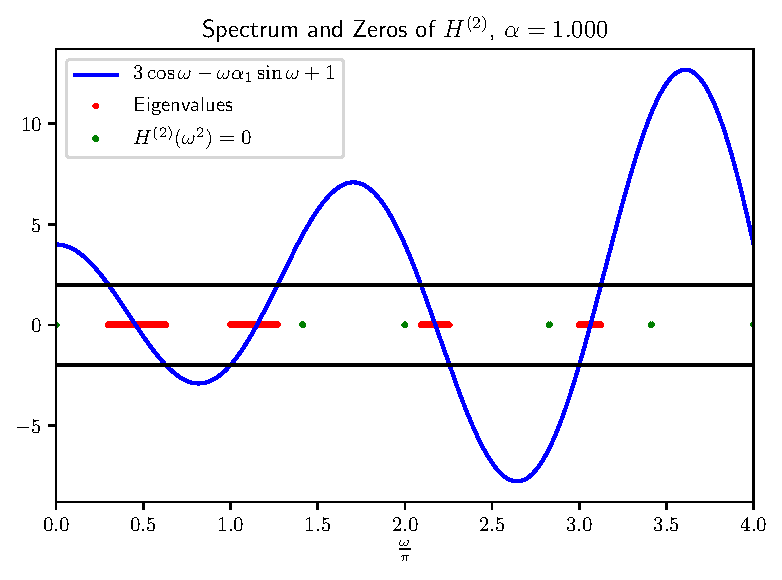
\includegraphics[scale=0.5]{1DDecoratedGraph_alpha1.pdf}
		\caption{\label{fig:1DDecoratedGraph_alpha1} The values of $\omega$ which solve \eqref{eq:EmbeddedGraphDetSolveCondition} with $\alpha_1=1$. No zeros of $H^{(2)}$ form part of the spectrum in this case.}
	\end{subfigure}
	~
	\begin{subfigure}[t]{0.45\textwidth}
		\centering
		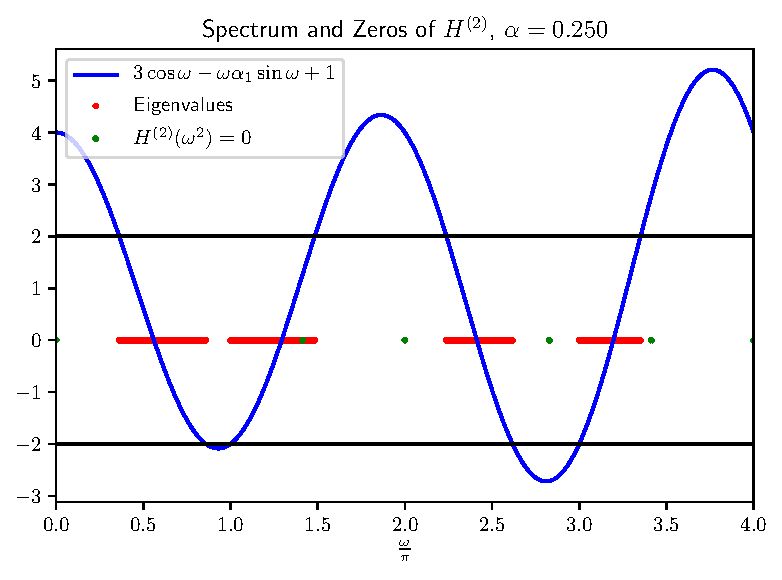
\includegraphics[scale=0.5]{1DDecoratedGraph_alpha0-25.pdf}
		\caption{\label{fig:1DDecoratedGraph_alpha0-25} The values of $\omega$ which solve \eqref{eq:EmbeddedGraphDetSolveCondition} with $\alpha_1=\recip{4}$. With $\alpha_1$ this small, some of the zeros of $H^{(2)}$ form part of the spectrum.}
	\end{subfigure}
	\caption{\label{fig:1DDecoratedGraph} The values of $\omega$ which solve \eqref{eq:EmbeddedGraphDetSolveCondition}, using $a=\recip{\sqrt{2}}$. Changing the value of $\alpha$ effects how many zeros of $H^{(2)}$ are included in the spectrum.}
\end{figure}
Zeros of $H^{(2)}$ occur at $\omega= 2n\pi, \frac{n\pi}{a}, \frac{n\pi}{b}$, which also solve \eqref{eq:EmbeddedGraphDetSolveCondition} for all values of $\qm$.
Examining the limit \eqref{eq:EigenvalueBranchLimit} reveals that if $H^{(2)}\bracs{\omega_0^2}=0$, $\omega_0$ is part of the spectrum only when there exists a $\qm_0\in\left[-\pi,\pi\right)$ such that $\Xi\bracs{\omega_0}=\cos\theta_0+\recip{2}$.
That is, the bracketed term in \eqref{eq:EmbeddedGraphDetSolveCondition} is required to be zero for a root of $H^{(2)}$ to be part of the spectrum.
The eigenvalue branches in the vicinity of root $\omega_0=\pi\sqrt{2}$ are plotted in figure \ref{fig:1DDecoratedGraphEvalBranches-Thetas}, to illustrate this point.
\begin{figure}[t!]
	\centering
	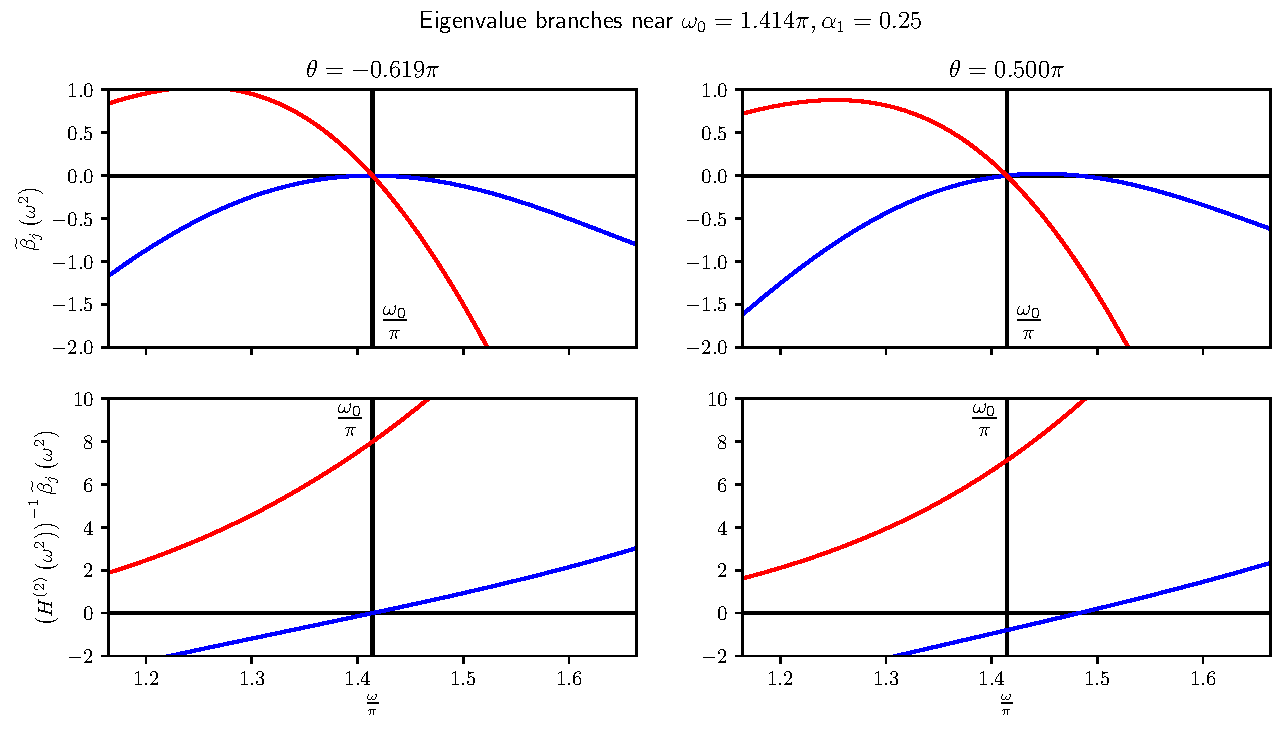
\includegraphics[scale=0.7]{1DDecoratedGraphEvalBranches-Thetas.pdf}
	\caption{\label{fig:1DDecoratedGraphEvalBranches-Thetas} eigenvalue branches of the matrix $\mathfrak{M}_{\qm}$ near $\omega_0 = \pi\sqrt{2}$, which is a root of $H^{(2)}$. The value $\qm_0\approx-0.691\pi$ solves $\Xi\bracs{\omega_0}=\cos\qm_0+\recip{2}$, and the limit \eqref{eq:EigenvalueBranchLimit} is zero. At other values of $\qm$ however, the limit \eqref{eq:EigenvalueBranchLimit} is non-zero.}
\end{figure}
It is also worth noting that (in figure \ref{fig:1DDecoratedGraphEvalBranches-Thetas}) there are two eigenvalue branches which are zero at $\omega_0$, with the third being non-zero at $\omega_0$.
For both branches, the limit \eqref{eq:EigenvalueBranchLimit} exists, however only for one is it zero.
The spectrum of \eqref{eq:SingularScalarWaveEqnWholeSpace} thus consists of those $\omega^2$ such that
\begin{align*}
	\abs{ 3\cos\omega - \alpha_1\omega\sin\omega + 1 } \leq 2.
\end{align*}
As expected, the spectrum does not depend on $\beta$ despite the fact that the $M$-matrix for each operator on $\graph_{\mathcal{P}}$ does.
It does differ from the spectrum of the quantum graph in section \ref{ssec:Example1DLoop} due to the presence of the ``decoration" $I_{12}$, although this difference only depends on the length this additional edge.

\subsection{Cross in the Periodic Plane} \label{ssec:ExampleCrossInPlane}
Our final example is a two-dimensional graph whose period cell represents a lattice-like structure in $\reals^2$.
Consider the embedded, periodic graph defined as follows --- for each $\bracs{n,m}\in\integers^2$ define
\begin{align*}
	v^{(n,m)} &= \bracs{n+\recip{2}, m+\recip{2}}, \quad
	I_{\mathrm{left}}^{\bracs{n,m}} = \sqbracs{v^{\bracs{n,m}}, v^{\bracs{n+1,m}}}, \quad
	I_{\mathrm{up}}^{\bracs{n,m}} = \sqbracs{v^{\bracs{n,m}}, v^{\bracs{n,m+1}}}, \\
	\vertSet^* &= \clbracs{v^{\bracs{n,m}} \setVert \bracs{n,m}\in\integers^2}, \quad
	\edgeSet^* = \clbracs{ I_{\mathrm{l}}^{\bracs{n,m}}, I_{\mathrm{u}}^{\bracs{n,m}} \setVert \bracs{n,m}\in\integers^2}, \quad
	\graph^* = \bracs{\vertSet^*, \edgeSet^*}.
\end{align*}
Place a coupling constant $\alpha^{\bracs{n,m}} =: \alpha_3>0$ at each $v^{(n,m)}$.
The period graph of $\graph^*$ occupies $\left[0,1\right)^2$ and consists of a single vertex with two looping edges of length 1.
Breaking the loops by introducing two artificial vertices takes us to the quantum graph
\begin{align*}
	\vertSet = \clbracs{v_1, v_2, v_3}, \quad
	\edgeSet = \clbracs{I_{13}, I_{31}, I_{23}, I_{32}}, \quad
	\graph = \bracs{\vertSet, \edgeSet},
\end{align*}
with
\begin{align*}
	l_{13} = b, \quad l_{31} = \tilde{b} := 1-b, \quad 
	l_{23} = a, \quad l_{32} = \tilde{a} := 1-a, \qquad
	\qm_{13} = \qm_{31} = \qm_2, \quad \qm_{23} = \qm_{32} = \qm_1,
\end{align*}
and coupling constant $\alpha_3$ at $v_3$ (and zero coupling constants at the dummy vertices $v_1$ and $v_2$).
Also define
\begin{align*}
	 s_a\bracs{\omega} = \sin\bracs{a\omega}, \quad 
	 c_a\bracs{\omega} = \cos\bracs{a\omega}, \quad 
	 s_b\bracs{\omega} = \sin\bracs{b\omega}, \quad 
	 c_b\bracs{\omega} = \cos\bracs{b\omega},
\end{align*}
\begin{align*}
	 \tilde{s}_a\bracs{\omega} = \sin\bracs{\omega\bracs{1-a}}, \quad 
	 \tilde{c}_a\bracs{\omega} = \cos\bracs{\omega\bracs{1-a}}, \quad 
	 \tilde{s}_b\bracs{\omega} = \sin\bracs{\omega\bracs{1-b}}, \quad 
	 \tilde{c}_b\bracs{\omega} = \cos\bracs{\omega\bracs{1-b}}.
\end{align*}
Using corollary \ref{cory:M-MatrixEntriesNoPoles} we set $H^{(2)}\bracs{\omega^2} = s_a\bracs{\omega} s_b\bracs{\omega} \tilde{s}_a\bracs{\omega} \tilde{s}_b\bracs{\omega}$, and obtain
\begin{align*}
	\mathfrak{M}_{\qm}\bracs{\omega^2} &=
	\begin{pmatrix}[2.5]
		-\omega s_a \tilde{s}_a \bracs{ s_b \tilde{c}_b + c_b \tilde{s}_b } &
		0 &
		\begin{split}
			&\omega s_a \tilde{s}_a \bracs{ e^{\rmi\qm_2\tilde{b}}s_b + e^{-\rmi\qm_2 b}\tilde{s}_b }
		\end{split} \\
		0 &
		-\omega s_b \tilde{s}_b \bracs{ s_a \tilde{c}_a + c_a \tilde{s}_a } &
		\begin{split}
			&\omega s_b \tilde{s}_b \bracs{ e^{\rmi\qm_1\tilde{a}}s_a + e^{-\rmi\qm_1 a}\tilde{s}_a } 
		\end{split} \\
		\omega s_a \tilde{s}_a \bracs{ e^{-\rmi\qm_2\tilde{b})}s_b + e^{\rmi\qm_2 b}\tilde{s}_b } &
		\omega s_b \tilde{s}_b \bracs{ e^{-\rmi\qm_1\tilde{a}}s_a + e^{\rmi\qm_1 a}\tilde{s}_a } &
		\begin{split}
			&-\omega ( s_a s_b \tilde{s}_a \tilde{c}_b 
			+ s_a s_b \tilde{c}_a \tilde{s}_b \\ 
			& + s_a c_b \tilde{s}_a \tilde{s}_b
			+ c_a s_b \tilde{s}_a \tilde{s}_b \\
			& - \omega\alpha_3 s_a s_b \tilde{s}_a \tilde{s}_b )
		\end{split}
	\end{pmatrix}.
\end{align*}
Examining \eqref{eq:QGDetSolveCondition} yields
\begin{align} \label{eq:ExampleThickVertexSolution}
	0 = \omega^3 s_a^2\bracs{\omega} s_b^2\bracs{\omega} \tilde{s}_a^2\bracs{\omega} \tilde{s}_b^2\bracs{\omega} \sin\bracs{\omega} 
	\bracs{ 4\cos\bracs{\frac{\qm_1+\qm_2}{2}}\cos\bracs{\frac{\qm_1-\qm_2}{2}} + \omega\alpha_3\sin\omega - 4\cos\omega}.
\end{align}
For ease, we define
\begin{align*}
	\Xi\bracs{\omega} := \cos\omega - \frac{\alpha_3\omega}{4}\sin\omega.
\end{align*}
From here, the analysis is similar to that of example \ref{ssec:EmbeddingDependentExample} --- any root of $H^{(2)}$ solves \eqref{eq:ExampleThickVertexSolution}, in addition to those $\omega$ for which $-1\leq\Xi\bracs{\omega}\leq 1$.
Examination of the eigenvalue branches then produces a familiar conclusion; if $H^{(2)}\bracs{\omega_0^2}=0$, $\omega_0$ forms part of the spectrum of \eqref{eq:SingularWaveEqnQGProblem} on $\graph$ if and only if there exists a $\qm_0$ such that the bracket in \eqref{eq:ExampleThickVertexSolution} is zero at $\bracs{\omega_0,\qm_0}$ -- that is if 
\begin{align} \label{eq:ExampleThickVertexSolutionReduced}
	\Xi\bracs{\omega}=\cos\bracs{\frac{\qm_1+\qm_2}{2}}\cos\bracs{\frac{\qm_1-\qm_2}{2}}.
\end{align}
As a result, the spectrum consists of exactly those $\omega$ such that
\begin{align*}
	-1 \leq \cos\omega - \frac{\alpha_3\omega}{4}\sin\omega \leq 1.
\end{align*}
In addition to recovering the spectrum of \eqref{eq:SingularWaveEqnQGProblem}, we can use \eqref{eq:ExampleThickVertexSolution} and \eqref{eq:QGGenEvalSolveNoPoles} to recover the eigenfunctions too.
For a given $\qm$, equation \eqref{eq:ExampleThickVertexSolutionReduced} can be solved for (a solution) $\omega=\omega_0$.
This $\omega_0$ corresponds to an eigenvalue $\omega_0^2$ of \eqref{eq:SingularWaveEqnQGProblem}, but also implies that there exists a $w\in\complex^{\abs{\vertSet}}$ such that \eqref{eq:QGGenEvalSolveNoPoles} holds at $\omega=\omega_0$.
Given that we can compute $\mathfrak{M}_{\qm}\bracs{\omega_0^2}$, and we \emph{know} $\mathfrak{M}_{\qm}\bracs{\omega_0^2}$ has a zero eigenvalue, it is not hard to (numerically) determine the associated eigenvector(s) $w$.
By definition of $\mathfrak{M}_\qm$ and the $M$-matrix, this vector $w = \dmap u$ is the Dirichlet data of the eigenfunction $u$ that corresponds to the eigenvalue $\omega_0^2$.
Given \eqref{eq:EdgeEqnGeneralSolution} and $w$, it is thus possible to reconstruct each of the edge functions $u^{(jk)}$ --- some examples of the result of this process are plotted in figure \ref{fig:CrossInPlane-EdgePlot}.
\begin{figure}[h!]
	\begin{subfigure}[t]{0.45\textwidth}
		\centering
		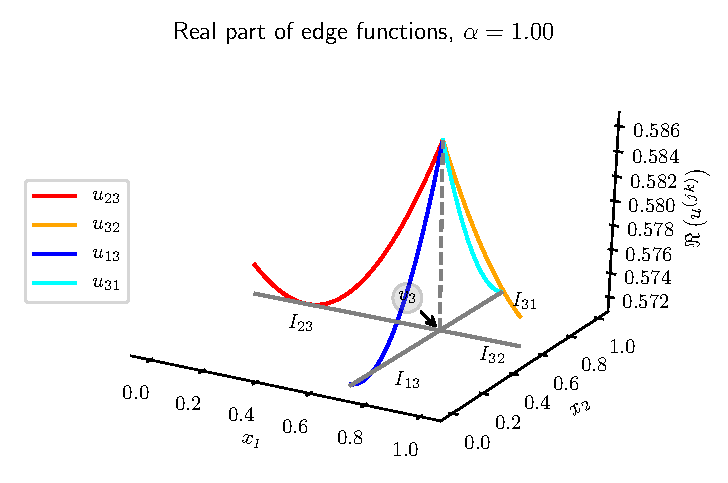
\includegraphics[scale=0.6]{CrossInPlane_EdgePlot-R-a1.pdf}
		\caption{\label{fig:CrossInPlane_EdgePlot-R-a1} The real part of the eigenfunction when $\omega_0=0.63936, \alpha=1$.}
	\end{subfigure}
	~
	\begin{subfigure}[t]{0.45\textwidth}
		\centering
		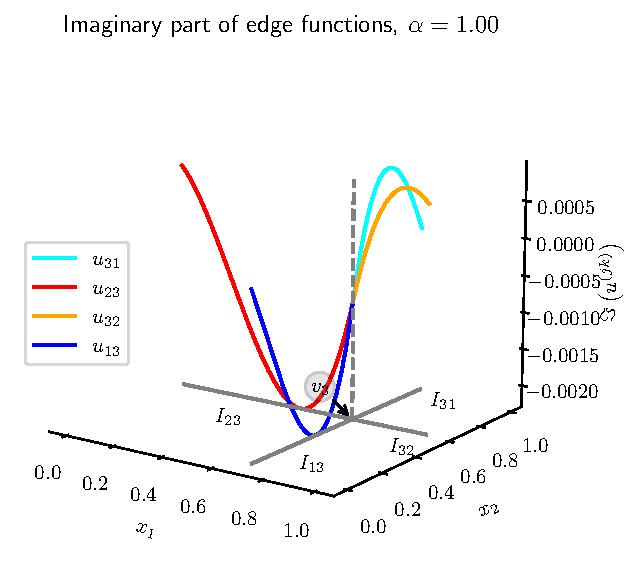
\includegraphics[scale=0.6]{CrossInPlane_EdgePlot-I-a1.pdf}
		\caption{\label{fig:CrossInPlane_EdgePlot-I-a1} The imaginary part of the eigenfunction when $\omega_0=0.63936, \alpha=1$.}
	\end{subfigure}
	\vskip\baselineskip
	\begin{subfigure}[t]{0.45\textwidth}
		\centering
		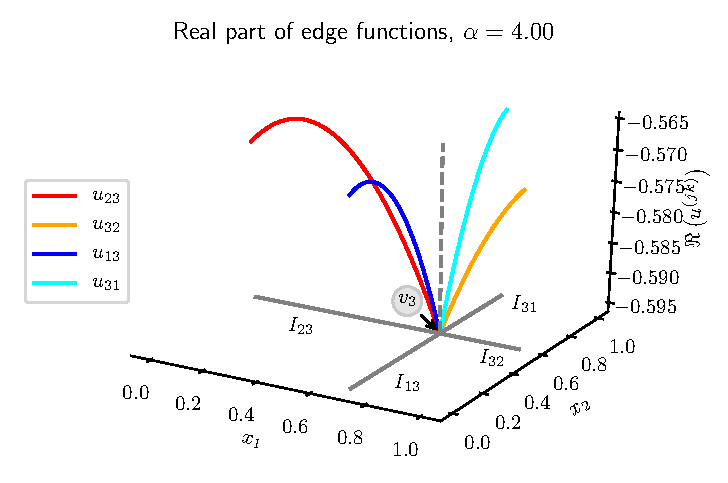
\includegraphics[scale=0.6]{CrossInPlane_EdgePlot-R-a4.pdf}
		\caption{\label{fig:CrossInPlane_EdgePlot-R-a4} The real part of the eigenfunction when $\omega_0=0.44812, \alpha=4$.}
	\end{subfigure}
	~
	\begin{subfigure}[t]{0.45\textwidth}
		\centering
		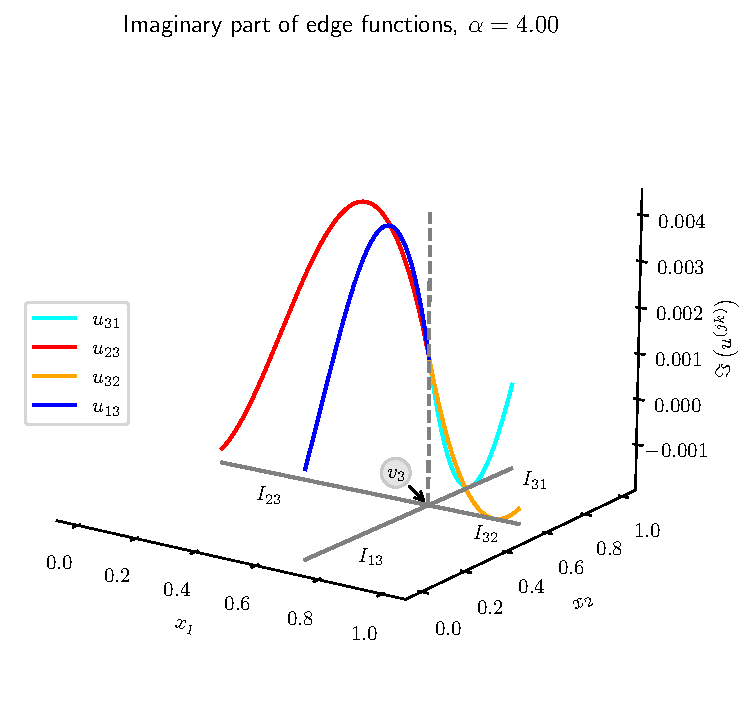
\includegraphics[scale=0.6]{CrossInPlane_EdgePlot-I-a4.pdf}
		\caption{\label{fig:CrossInPlane_EdgePlot-I-a4} The imaginary part of the eigenfunction when $\omega_0=0.44812, \alpha=4$.}
	\end{subfigure}	
	\caption{\label{fig:CrossInPlane-EdgePlot} Plots of the eigenfunction corresponding to the eigenvalue $\omega_0=0.63936$  when $\alpha=1$, and $\omega_0=0.44812$ when $\alpha=4$. Both eigenvalues are attained when $\qm=\bracs{\frac{\pi}{4},\frac{\pi}{4}}^\top$, and the edge functions are plotted above the graph $\graph$ in the $\bracs{x_1,x_2}$-plane.}
\end{figure}

To round off the analysis, quantities such as the integrated density of states (IDoS) and density of states (DoS) can also be estimated from \eqref{eq:ExampleThickVertexSolution}, shown in figure \ref{fig:CrossInPlane_ScalarDoS}, displaying the band-gap structure of the spectrum and demonstrating that the eigenvalues ``concentrate" at the center of each spectral band.
\begin{figure}[t!]
	\begin{subfigure}[t]{0.45\textwidth}
		\centering
		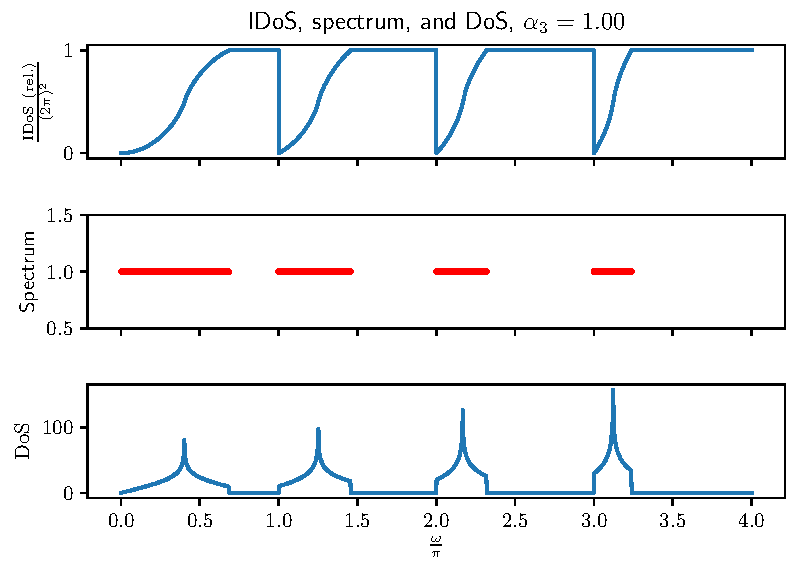
\includegraphics[scale=0.5]{CrossInPlane_ScalarDoS_alpha1-00.pdf}
		\caption{\label{fig:CrossInPlane_ScalarDoS_alpha1-00} The (relative) integrated density of states (IDoS), density of states (DoS) and spectrum for the system with $\alpha_3=1$.}
	\end{subfigure}
	~
	\begin{subfigure}[t]{0.45\textwidth}
		\centering
		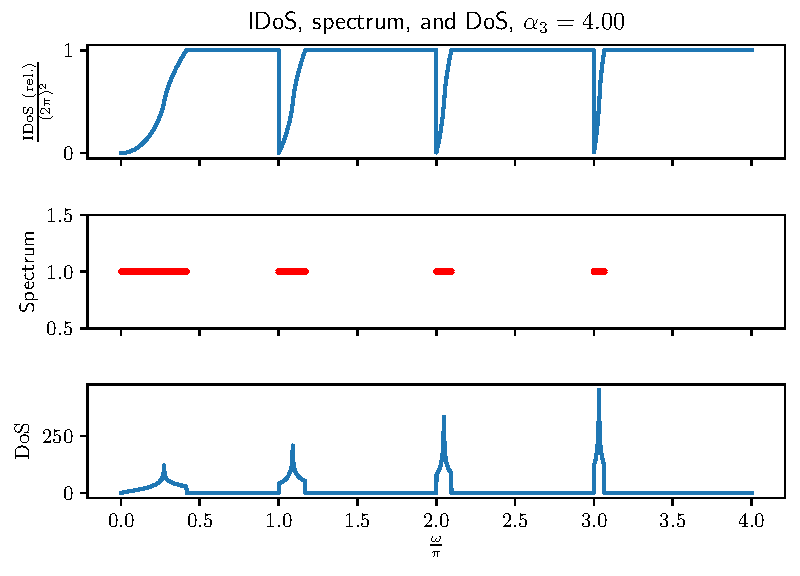
\includegraphics[scale=0.5]{CrossInPlane_ScalarDoS_alpha4-00.pdf}
		\caption{\label{fig:CrossInPlane_ScalarDoS_alpha4-00} The (relative) integrated density of states (IDoS), density of states (DoS) and spectrum for the system with $\alpha_3=4$.}
	\end{subfigure}	
	\caption{\label{fig:CrossInPlane_ScalarDoS} The (relative) IDoS, DoS, and spectrum for the graph topology in section \ref{ssec:ExampleCrossInPlane}.
	The relative IDoS at the value $x$ is defined as the IDoS at the value $x$ minus $\left\lfloor\frac{x}{\pi}\right\rfloor\bracs{2\pi}^2$.}
\end{figure}
For any $\alpha_3>0$, it can also be shown that the spectral bands $I_n$ satisfy $I_n\subset\sqbracs{(n-1)\pi, n\pi}$, each with left-endpoint $(n-1)\pi$ and a right-endpoint strictly less than $n\pi$.
It is worth remarking that this behaviour is reversed for $\alpha_3<0$, the bands having right-endpoint $n\pi$ and left-endpoint strictly greater than $(n-1)\pi$.
For $\alpha\leq-2$ there is even a gap between an isolated eigenvalue at $0$ and the beginning of the band $I_1$ --- however as mentioned in section \ref{sec:ScalarEqnChapterIntro}, $\alpha<0$ does not correspond to any physical material.
This result is consistent with similar applications of singular-structures as approximations to thin-material structures, like the work of \cite{cherednichenko2019time}, in which the natural physical constraints on the parameters in the problem prevent a similar opening of a band-gap at the bottom of the spectrum.


% Conclusions, including motivation for curved edges
\section{Concluding Remarks} \label{sec:Scalar-Conc}
The work of this chapter provides us with a foundation to build upon, as we turn our attention towards problems motivated by the equations of electromagnetism and towards domains that better reflect composite materials.

Our analysis in section \ref{sec:3DGradSobSpaces} provides us with an understanding, both intuitively and rigorously, of the gradient-like objects that our variational problem requires us to work with.
We have seen that gradients of zero emerge due to our singular measures inability to determine the behaviour of functions on $\ddom$ outside $\graph$, and that the tangential gradient corresponds to the derivative -- the one dimensional analogue of the gradient --- directed along each of the edges of $\graph$.
This is an intuitive and expected behaviour; the singular measure $\dddmes$ only respects one dimensional lengths along $\graph$, effectively throwing away the information in the direction normal to the edges of $\graph$, and as a result the two dimensional gradient is replaced with the (essentially) one dimensional tangential gradient.
For gradients this one-dimensional analogue is fairly easy to accept, however there is no such analogue for the curl (or divergence) operator acting on a vector field.
That being said, the analysis of $\ktgradSob{\ddom}{\dddmes}$ has also provided us with the method to employ in identifying what the notion of curl (and to an extent divergence) should be, which will be the focus of section \ref{sec:CC-CurlAnalysis}.
Our knowledge of $\ktgradSob{\ddom}{\dddmes}$ will also prove valuable in chapter \ref{ch:SingInc}, when we reintroduce the background material that surrounds the graph $\graph$.

Section \ref{sec:ScalarDerivation} establishes the link between the singular structure problem \eqref{eq:SingularScalarWaveEqn} and the class of problems that emerge in the zero-thickness limit of thin structures.
The coupling constants $\alpha_j$ take on the role of the ratio of vertex-to-edge volumes (see section \ref{ssec:Intro-ThinStructures}), that is the parameters quantifying the geometric contrast in the thin structures.
We also observed how the space $\tgradSob{\ddom}{\dddmes}$ allows us to define operators ($-\laplacian_{\dddmes}^{\qm}$) corresponding to these limiting problems, through bilinear forms motivated by analogy with the weak formulation of the classical acoustic equation.
Both the construction of $\tgradSob{\ddom}{\dddmes}$ and the variational problem \eqref{eq:SingularScalarWaveEqn} were motivated by the simplicity of the ``visual" limit of a thin-structure and analogy with the classical acoustic approximation.
Exploring this analogy has provided us with an effective tool for the definition of the extended spaces and operators that one obtains in this limit.
Exploring the extent of this analogy will be the motivation behind the variational problems we will come to consider in chapters \ref{ch:CurlCurl} and \ref{ch:SingInc}; we have seen that our approach coincides with known results for the acoustic approximation on thin structures in the zero-thickness limit, and we now ask whether our approach can be used as a predictive tool for the curl of the curl problem, and for the limit of a composite material.

Our derivation in section \ref{sec:ScalarDerivation} also allows us to use the theory surrounding the $M$-matrix for explicitly determining the spectrum of $-\laplacian_{\dddmes}^{\qm}$, as discussed in section \ref{sec:ScalarDiscussion}.
It is reiterated here that a formal analysis in the use of the $M$-matrix for the solution of problems bearing generalised resolvents has yet to be carried out (see section \ref{sec:ScalarDiscussion}).
We have provided an explicit expression for the $M$-matrix of \eqref{eq:SingularWaveEqnQGProblem} on any finite, connected, periodic graph and discussed a number of considerations when using the $M$-matrix to analyse the spectrum.
Our discussion points are complimented with the examples of section \ref{sec:ScalarExamples}; including how one can also gain access to the eigenfunctions and (integrated) density of states (section \ref{ssec:ExampleCrossInPlane}), the necessity of artificial vertices (section \ref{ssec:Example1DLoop}), and how potential freedoms in the choice of embedding for a quantum graph do not affect the resulting spectrum (section \ref{ssec:EmbeddingDependentExample}).

Before we move on to considering the analogue of the curl-of-the-curl equation (chapter \ref{ch:CurlCurl} and composite domains with singular components (chapter \ref{ch:SingInc}), we highlight the possibility of extending the analysis carried out thus far to embedded graphs whose edges are not assumed to be straight line segments, and to accommodate the presence of external fields.

\subsection{Extensions: Curved Edges and Potential Fields} \label{ssec:CurvedEdges}
Our analysis has been, and in the following chapters will continue to be, carried out within the context of the standing assumptions \ref{ass:MeasTheoryProblemSetup} --- this in particular enforces the edges of our singular structure are straight lines.
However the inclusions within the periodic cross sections of physical photonic crystals, and the thin structure systems modelled by quantum graphs, are not limited to unions of straight edges.
With our analysis of $\gradZero{\ddom}{\dddmes}$ and $\ktgradSob{\ddom}{\dddmes}$ complete, we can articulate on some of the changes to the arguments one would need to make, and the resulting changes to the realisation \eqref{eq:SingularWaveEqnQGProblem} one would obtain.

To this end, let us now suppose that the edges $I_{jk}$ of our (period) graph $\graph$ are (continuous) curves in $\ddom$.
We know that, when our graph consists of straight edges, that tangential gradients are directed along the edges $I_{jk}$ and gradients of perpendicular to the edges.
Nothing in this geometric understanding changes when moving from straight to curved edges --- we should still expect tangential gradients to point ``along" the edges $I_{jk}$.
Indeed, the (now curved) edges $I_{jk}$ are still related to the intervals $\sqbracs{0,l_{jk}}$, it is simply the case now that the vector $e_{jk}$ is no longer constant along $I_{jk}$.
However we also remark that the vector $e_{jk}$ being no longer constant means that the quasi-momentum-related terms $\qm_{jk}$ are now \emph{also} non constant.
As such, we should expect that
\begin{align*}
	\tgrad_{\lambda_{jk}}u(x) = \bracs{ u_{jk}'(y) + \rmi\qm_{jk}(y) u_{jk}(y)}e_{jk}(y),
	\qquad x = r_{jk}(y),
\end{align*}
where $r_{jk}:\interval{l_{jk}}\rightarrow I_{jk}$ is the (measure-preserving) parametrisation of the curve $I_{jk}$, and $e_{jk}(y) = r_{jk}'(y)$ is the direction tangential to the edge $I_{jk}$ at the point $y$, and $\qm_{jk}(y)=\qm\cdot e_{jk}(y)$.
We make these predictions not only because of the geometric interpretations we now have for tangential gradients (and gradients of zero), but because the arguments of section \ref{sec:3DGradSobSpaces} do not depend on our requirement that $I_{jk}$ be straight, \emph{except} when we come to identify the explicit form for gradients of zero and tangential gradients on our edges.
Of course there are some technicalities to overcome --- the smoothness of the curves $I_{jk}$ will affect how one goes about constructing explicit approximating sequences for determining gradients of zero, for example.

Further to these expectations, one would expect to obtain a system of the form
\begin{subequations} \label{eq:SS-QGProblemCurvedEdges}
	\begin{align}
		-\bracs{\diff{}{y} + \rmi\qm_{jk}(y)}^2 u^{(jk)} &= \omega^2 u^{(jk)}, \quad &y\in\interval{l_{jk}}, \ \forall I_{jk}\in\edgeSet, \label{eq:SS-QGProblemCurvedEdges-1} \\
		u \text{ is continuous at } & v_j, \quad &\forall v_j\in\vertSet,  \\
		\sum_{j\con k}\bracs{\pdiff{}{n} + \rmi\qm_{jk}(v_j)}u^{(jk)}\bracs{v_j} &= \omega^2\alpha_j u\bracs{v_j}, \quad &\forall v_j\in\vertSet,
	\end{align}
\end{subequations}
in place of the system \eqref{eq:SingularWaveEqnQGProblem}).
This new system is still realisable as a quantum graph problem, however we now have co-ordinate varying coefficients (through the $\qm_{jk}(y)$) in our edge ODEs.
The Green's identity still holds for the operator that defines the problem \eqref{eq:SS-QGProblemCurvedEdges}, with the Dirichlet map as defined in \eqref{eq:GraphDNMapDef} and Neumann map defined as
\begin{align*}
	\bracs{\nmap u}_j &= \sum_{j\con k} \bracs{ \pdiff{}{n} + \rmi\qm_{jk}(v_j) }u(v_j) .
\end{align*}
One can thus construct the $M$-matrix for this problem and attempt to use it to analyse the spectrum, however an explicit form for the entries is greatly complicated by the $y$-dependence of the $\qm_{jk}$.
The proof of proposition \ref{prop:M-MatrixEntries} relies on being able to compute the general solution to \eqref{eq:SS-QGProblemCurvedEdges-1}, which is now a non-trivial task for general functions $\qm_{jk}(y)$.
Further investigation into possible alternatives, or the viability of solving via the $M$-matrix, would be warranted.

Following on from the above discussion, the system \eqref{eq:SS-QGProblemCurvedEdges} resembles that of the magnetic Schr\"{o}dinger operator on a graph --- see \cite[section 7.5.1]{berkolaiko2013introduction} --- although the coefficients $\qm_{jk}$ a mixture of the geometry of our structure and the use of the Gelfand transform.
This observation brings a further generalisation to \eqref{eq:SingularScalarWaveEqn} to light, that is within immediate reach --- the introduction of (to use the terminology from the Schr\"{o}dinger context) a magnetic field $\vec{A}$ and potential $V$, and consideration of a variational problem such as
\begin{align*}
	\integral{\ddom}{ \bracs{\tgrad_{\dddmes}u + \vec{A}u}\cdot \overline{\bracs{ \tgrad_{\dddmes}\phi + \vec{A}\phi}} + Vu\overline{\phi} }{\dddmes} 
	&= \omega^2\integral{\ddom}{u\overline{\phi}}{\dddmes},
	\qquad \forall\phi\in\psmooth{\ddom}.
\end{align*}
The analysis of section \ref{sec:3DGradSobSpaces} continues to provide us with an understanding of the objects involved in this variational problem --- we can even draw the immediate conclusion that $\vec{A}$ must be parallel to each edge on $I_{jk}$ by testing against gradients of zero.
However the method of solving such a problem will likely bear all of the challenges the previous discussion raised, if not more.

% Indicate that the appendix has now begun
\begin{subappendices}

% Theory for tangential gradients
\section{Sobolev Spaces of Functions with Gradients} \label{ssec:3DGradSobSpaces}
\tstk{proper introductory section here? Also, need to change from $x_1$-parallel to $x_2$-parallel throughout! Otherwise things are going to get really annoying}

\tstk{have done some setup to be able to lead with...}

Thematic throughout our analysis of gradients of zero and Sobolev functions will be the following procedure; we will first aim to understand gradients of zero on a single edge $I_{jk}$ that is parallel to (one of) the co-ordinate axes, and then employ rotation ideas to generalise our arguments to edges at any angle to the axes.
Next, we demonstrate that gradients of zero on $\graph$ can be built up from those on the individual edges --- this is unsurprising given that $\ddmes$ is just the sum of the individual singular measures supporting each edge.
Once we understand gradients of zero on edges, we can then understand the tangential gradients on the edges and on $\graph$ by following a similar line of reasoning --- working on the edges first and then looking at the implications for functions on the entire graph.
We will also have to consider (and analyse) the behaviour of gradients of zero and tangential gradients at the vertices, induced by $\nu$.
This finally allows us to understand Sobolev functions and their tangential gradients (and gradients of zero) on $\graph$ with respect to the measure $\dddmes$.
This approach will also guide us when we come to examine the Sobolev spaces of curls in section \tstk{ref!}.

As promised, we begin with an examination of gradients of zero. \tstk{we will come to consider $\kappa$-gradients in a later chapter, so to save time we might as well deal with them here. We can set $\kappa=0$, or ignore the third component in this section without any harm coming to us.}

\subsection{Gradients of Zero} \label{ssec:muGradZero}
In this section we will characterise gradients of zero with respect to the measures $\ddmes, \nu$, and $\dddmes$, in that order.
Throughout, we denote by $\ograd$ the $\ktgrad$ operator with $\kt=\bracs{0,0}$.
Given proposition \ref{prop:ZeroInvariantUnderQM-Wavenumber}, without loss of generality we can always take any approximating sequence $\phi_n$ for a gradient of zero $g$ to be such that $\ograd\phi_n\rightarrow g$, as opposed to $\ktgrad\phi_n\rightarrow g$.
\begin{prop}[Gradients of Zero on a Segment Parallel to the $x_2$-axis] \label{prop:3DGradZeroParallel}
	Suppose that the edge $I_{jk}$ is parallel to the $x_2$-axis.
	Then 
	\begin{align*}
		\gradZero{\ddom}{\lambda_{jk}} &= 
		\clbracs{ \bracs{g,0,0}^\top	\setVert g\in\ltwo{\ddom}{\lambda_{jk}} }.
	\end{align*}
\end{prop}
\begin{proof}
	This is a version of the argument in \cite[Section~3.1]{zhikov2000extension}, given proposition \ref{prop:GradZeroInvarientUnderQM} we can consider (without loss of generality) $\kt=\bracs{0,0}$ throughout.
	This argument is also one particular version of the argument in the proof of proposition \ref{prop:RotationOfEdgeGradients}, which we present in detail below.
\end{proof}

\begin{prop} \label{prop:3DGradZeroRotated}
	Let $I_{jk}$ be an edge of $\graph$.
	Then
	\begin{align*}
		\gradZero{\ddom}{\lambda_{jk}} 
		&= \clbracs{ g_{jk}\hat{n}_{jk} \setVert g_{jk}\in\ltwo{\ddom}{\lambda_{jk}} } \\
		&= \clbracs{ \begin{pmatrix} R_{jk}^{\top} & 0 \\ 0 & 1 \end{pmatrix} \bracs{g_{jk},0,0}^\top \setVert g_{jk}\in\ltwo{\ddom}{\lambda_{jk}} } \\
		&= \clbracs{ g_{jk}\in\ltwo{\ddom}{\ddmes}^2 \setVert g_{jk}\cdot e_{jk} = 0 }.
	\end{align*}
\end{prop}
Note that the three sets on the right hand side are all equal by definition of $n_{jk}, e_{jk}$, and $R_{jk}$.
As such, we will demonstrate the equality on the first line in the proof. 
\begin{proof}
	Clearly, if $g=\bracs{0,0,g_3}^\top\in\gradZero{\ddom}{\lambda_{jk}}$, then \eqref{eq:GradZeroSequenceDef} implies that $g_3=0$.
	
	Next, suppose that $g=g_{jk}\hat{e}_{jk}\in\gradZero{\ddom}{\lambda_{jk}}$, and take an approximating sequence $\phi_n$ for $g$.
	Given proposition \ref{prop:ZeroInvariantUnderQM-Wavenumber}, this implies that
	\begin{align*}
		\phi_n\lconv{\ltwo{\ddom}{\lambda_{jk}}}0, \quad
		\ograd\phi_n \lconv{\ltwo{\ddom}{\lambda_{jk}}^3} g\hat{e}_{jk}.
	\end{align*}
	Therefore, $\ograd\phi_n\cdot\hat{e}_{jk}\rightarrow g$, and thus
	\begin{align*}
		\int_0^{\abs{I_{jk}}} \abs{\diff{\phi_n}{y}\bracs{r_{jk}(y)} - g\bracs{r_{jk}(y)} }^2 \ \md y
		&= \integral{I_{jk}}{ \abs{\ograd\phi_n\cdot\hat{e}_{jk} - g}^2 }{\lambda_{jk}} \toInfty{n}, \\
		\implies \diff{\phi_n}{y}\bracs{r_{jk}(y)} &\lconv{\ltwo{\interval{I_{jk}}}{y}} g\bracs{r_{jk}(y)}.
	\end{align*}
	We also observe that $\phi_n\bracs{r_{jk}(y)}\rightarrow 0$ in $\ltwo{\interval{I_{jk}}}{y}$, and thus $g\bracs{r_{jk}(y)}$ is the derivative (in the classical $\gradSob{\interval{I_{jk}}}{y}$-sense) of the zero function, and thus $g=0$.
	
	Finally, suppose that $g\in\smooth{\ddom}$ and consider the smooth function $\phi(x) = \bracs{\bracs{x-v_j}\cdot n_{jk}}g(x)$.
	Then we have that $\ograd\phi_n = \bracs{\bracs{x-v_j}\cdot n_{jk}}\ograd g + g\hat{n}_{jk}$, and notice that $\bracs{x-v_j}\cdot n_{jk}	=0$ when $x\in I_{jk}$.
	It is now clear that $\phi=0$ and $\ograd\phi = g\hat{n}_{jk}$ on $I_{jk}$, so $g\hat{n}_{jk}\in\gradZero{\ddom}{\lambda_{jk}}$.
	By density of $\smooth{\ddom}$ in $\ltwo{\ddom}{\lambda_{jk}}$, we can conclude that $g\hat{n}_{jk}\in\gradZero{\ddom}{\lambda_{jk}}$ for every $g\in\ltwo{\ddom}{\lambda_{jk}}$.
\end{proof}
Taking $R_{jk}$ as the identity matrix to recover proposition \ref{prop:3DGradZeroParallel}.

We now focus on demonstrating that the set of gradients of zero on the entirety of $\graph$ is formed from gradients of zero on each edge.
That is, we look to prove the following characterisation of $\gradZero{\ddom}{\ddmes}$:
\begin{prop}[Characterisation of $\gradZero{\ddom}{\ddmes}$] \label{prop:3DGradZeroChar}
	For an embedded graph $\graph$ in $\ddom$, we have that
	\begin{align*}
		\gradZero{\ddom}{\ddmes} &= \clbracs{ g\in\ltwo{\ddom}{\ddmes}^3 \setVert g^{(jk)}\in\gradZero{\ddom}{\lambda_{jk}} \ \forall I_{jk}\in\edgeSet }.
	\end{align*}
\end{prop}
We will denote $B := \clbracs{ g\in\ltwo{\ddom}{\ddmes}^3 \setVert g^{(jk)}\in\gradZero{\ddom}{\lambda_{jk}} \ \forall I_{jk}\in\edgeSet }$ for the time being.
In order to prove proposition \ref{prop:3DGradZeroChar} we will need some supporting results, however the argument can be sketched out like so.
Showing that $\gradZero{\ddom}{\ddmes}\subset B$ is straightforward due to the definition of $\ddmes$ and that the norms we are interested in are related:
\begin{align*}
	\norm{\cdot}_{\ltwo{\ddom}{\lambda_{jk}}} &\leq \norm{\cdot}_{\ltwo{\ddom}{\ddmes}}, \\
	\norm{\cdot}_{\ltwo{\ddom}{\ddmes}}^2 &= \sum_{v_j\in\vertSet}\sum_{j\conLeft k}\norm{\cdot}_{\ltwo{\ddom}{\lambda_{jk}}}^2.
\end{align*}
The reverse inclusion is slightly more technical due to the fact that we have to form an approximating sequence (that converges on all of $\graph$) from a set of approximating sequences that each converge on one particular edge.
However we cannot simply extend an approximating sequence on an edge $I_{jk}$ by zero to the whole graph (as it is no longer guaranteed to be smooth), so have to smooth this sequence to zero over some small region around $I_{jk}$.
This ``smoothing" requires us to always have some non-zero distance between the edge $I_{jk}$ and all other edges of $\graph$, which is a non-trivial process if the support of the approximating sequence is close to one of the vertices $v_j$ or $v_k$.
Having overcome this obstacle, one can show that any $g_{jk}\in\gradZero{\ddom}{\lambda_{jk}}$ \emph{can} be extended by zero to obtain a function $g\in\gradZero{\ddom}{\ddmes}$, and then using linearity of the subspace $\gradZero{\ddom}{\ddmes}$, the proof will be complete.

Before continuing, we introduce two families of smooth functions that we shall make use of during the proof of proposition \ref{prop:3DGradZeroChar}.
Let $\eta\in\smooth{\ddom}$ have the properties
\begin{align*}
	0 \leq \eta(x) \leq 1, \quad
	\eta(x) = 0 \text{ when } \abs{x} \leq 1, \quad
	\eta(x) = 1 \text{ when } \abs{x} \geq 2.
\end{align*}
Then define
\begin{align*}
	\eta_j(x) = \eta\bracs{x-v_j}, \quad
	\eta_j^n(x) = \eta_j\bracs{nx},
\end{align*}
which are both smooth functions by composition.
The functions $\eta_j^n$ will enable us to extend functions defined on one edge $I_{jk}$ to the whole of $\graph$ without worrying about proximity to the vertex $v_j$.
Notice that $\eta_j^n\rightarrow 1 \toInfty{n}$ in $\ltwo{\ddom}{\ddmes}$ since
\begin{align*}
	\integral{\ddom}{ \abs{\eta_j^n - 1}^2 }{\ddmes} &\leq
	\integral{ B_{2/n}\bracs{v_j} }{}{\ddmes}
	= \ddmes\bracs{ B_{2/n}\bracs{v_j} } \leq \frac{4\abs{\edgeSet}}{n}.
\end{align*}
Additionally, we have that $\eta_j^n$ also converges in $\ltwo{\ddom}{\dddmes}$ to the function
\begin{align*}
	\tilde{\charFunc{j}} = \begin{cases} 1 & x\neq v_j, \\ 0 & x=v_j, \end{cases}
\end{align*}
since
\begin{align*}
	\norm{\eta_j^n - \tilde{\charFunc{j}}}_{\ltwo{\ddom}{\ddmes}}^2
	&= \norm{\eta_j^n - 1}_{\ltwo{\ddom}{\ddmes}}^2
	+ \integral{\ddom\setminus\clbracs{v_j}}{ \abs{\eta_j^n - 1}^2 }{\nu} \\
	&= \norm{\eta_j^n - 1}_{\ltwo{\ddom}{\ddmes}}^2 \rightarrow 0.
\end{align*}
Unsurprisingly we also need a family of smooth functions to help us ``smooth off" any approximating sequences.
Let $I_{jk}\in\edgeSet$, $\eps>0$, and set
\begin{align} \label{eq:ShortenedEdgeDef}
	I_{jk}^\eps := \clbracs{ x\in I_{jk} \setVert \mathrm{dist}\bracs{x,\partial I_{jk}}\leq\recip{\eps} }.
\end{align}
Let $\chi_{jk}^\eps\in\smooth{\ddom}$ be such that
\begin{align*}
	0 \leq \chi_{jk}^n \leq 1, \quad
	\chi_{jk}^\eps(x) = 1 \text{ when } \mathrm{dist}\bracs{x, I_{jk}^\eps}\leq \recip{3\eps}, \quad
	\chi_{jk}^\eps(x) = 0 \text{ when } \mathrm{dist}\bracs{x, I_{jk}^\eps}\geq \frac{2}{3\eps}.
\end{align*}
As $\graph$ is finite, we can assume without loss of generality that the only edge of $\graph$ that $\supp\bracs{\chi_{jk}^\eps}$ intersect is $I_{jk}$ (otherwise, we just rescale the argument).
We can also assemble $\chi_{jk}^\eps$ such that $\abs{ \ograd\chi_{jk}^{\eps} } \leq c\eps$ for some $c\geq 0$ independent of $\eps$.
We can check the convergence of $\chi_{jk}^\eps \toInfty{\eps}$ in $\ltwo{\ddom}{\ddmes}$ to the characteristic function of the edge $I_{jk}$, denoted by $\charFunc{jk}$;
\begin{align*}
	\integral{\ddom}{ \abs{\chi_{jk}^\eps - \charFunc{jk}}^2 }{\ddmes}
	&= \integral{I_{jk}}{ \abs{\chi_{jk}^\eps - \charFunc{jk}}^2 }{\lambda_{jk}}
	\leq \integral{I_{jk}\cap\clbracs{\chi_{jk}^\eps\leq 1}}{}{\lambda_{jk}}
	= \frac{2}{3\eps} \rightarrow 0 \toInfty{\eps}.
\end{align*}
We also have that $\chi_{jk}^\eps$ converges to the characteristic function $\charFunc{jk}^\circ$ of the interior of $I_{jk}$ in $\ltwo{\ddom}{\dddmes}$, since
\begin{align*}
	\integral{\ddom}{ \abs{\chi_{jk}^\eps - \charFunc{jk}^\circ}^2 }{\dddmes}
	&= \integral{\ddom}{ \abs{\chi_{jk}^\eps - \charFunc{jk}^\circ}^2 }{\ddmes}
	= \integral{\ddom}{ \abs{\chi_{jk}^\eps - \charFunc{jk}}^2 }{\ddmes}.
\end{align*}

We can now prove proposition \ref{prop:3DGradZeroChar} --- the inclusion $\gradZero{\ddom}{\ddmes}\subset B$ follows immediately.
\begin{lemma} \label{lem:3DGradZeroSubsetB}
	\begin{align*}
		\gradZero{\ddom}{\ddmes} \subset B.
	\end{align*}
\end{lemma}
\begin{proof}
	This is a direct consequence of $\lambda_{jk}$ being a restriction of $\ddmes$ to a given edge.
	Indeed, let $g\in\gradZero{\ddom}{\ddmes}$ and let $\phi_n$ be an approximating sequence for $g$.
	Then clearly
	\begin{align*}
		\norm{\phi_n}_{\ltwo{\ddom}{\lambda_{jk}}} &\leq \norm{\phi_n}_{\ltwo{\ddom}{\ddmes}} \rightarrow 0, \\
		\norm{\ograd\phi_n - g^{(jk)}}_{\ltwo{\ddom}{\lambda_{jk}}} &\leq \norm{\ograd\phi_n - g}_{\ltwo{\ddom}{\ddmes}} \rightarrow 0,
	\end{align*}
	thus $g\in\ltwo{\ddom}{\lambda_{jk}}$ for every $I_{jk}$, so $g\in B$.
\end{proof}
Turning our attention to the reverse inclusion, we first demonstrate that so long as a gradient of zero on an edge $I_{jk}$ has support contained within the interior of the $I_{jk}$, we can extend it to a gradient of zero on the whole graph.
\begin{lemma}[Extension lemma for Gradients of Zero] \label{lem:3DExtensionLemmaGrads}
	Let $n\in\naturals$ and $I_{jk}^n$ be as in \eqref{eq:ShortenedEdgeDef}.
	Suppose that $g_{jk}\in\gradZero{\ddom}{\lambda_{jk}}$ with $\supp\bracs{g_{jk}}\subset I_{jk}^n$.
	Define the functions $g\in\ltwo{\ddom}{\ddmes}$ and $\tilde{g}\in\ltwo{\ddom}{\dddmes}$ by
	\begin{align*}
		g =	\begin{cases} g_{jk} & \mathrm{on} \ I_{jk}, \\ 0 & \mathrm{otherwise}, \end{cases} 
		&\quad
		\tilde{g} =	\begin{cases} g_{jk} & \mathrm{on} \ I_{jk}\setminus\clbracs{v_j,v_k}, \\ 0 & \mathrm{otherwise}. \end{cases}
	\end{align*}
	Then $g\in\gradZero{\ddom}{\ddmes}$ and $\tilde{g}\in\gradZero{\ddom}{\dddmes}$.
\end{lemma}
\begin{proof}
	Let $\phi_n$ be an approximating sequence for $g_{jk}$, and consider the sequence (of smooth functions) $\psi_l = \chi_{jk}^n\phi_l$.
	We have that
	\begin{align*}
		\norm{\psi_l}_{\ltwo{\ddom}{\ddmes}} 
		&= \norm{\chi_{jk}^n\phi_l}_{\ltwo{\ddom}{\lambda_{jk}}}
		\leq \norm{\phi_l}_{\ltwo{\ddom}{\lambda_{jk}}} \rightarrow 0 \toInfty{l}.
	\end{align*}
	Furthermore,
	\begin{align*}
		\norm{\ograd\psi_l - g}_{\ltwo{\ddom}{\ddmes}^2}^2
		&= \norm{\chi_{jk}^n\ograd\phi_l + \phi_l\ograd\chi_{jk}^n - g_{jk}}_{\ltwo{\ddom}{\lambda_{jk}}^2}^2 \\
		&\leq 2\norm{\phi_l\ograd\chi_{jk}^n}_{\ltwo{\ddom}{\lambda_{jk}}^2}^2 + 2\norm{\chi_{jk}^n\ograd\phi_l - g_{jk}}_{\ltwo{\ddom}{\lambda_{jk}}^2}^2 \\
		&\leq 2\sup_{I_{jk}}\abs{\ograd\chi_{jk}^n}^2 \norm{\phi_l}_{\ltwo{\ddom}{\lambda_{jk}}^2}^2
		+ 2\norm{\ograd\phi_l - g_{jk}}_{\ltwo{\ddom}{\lambda_{jk}}^2}^2 \\
		&\rightarrow 0 \toInfty{l}.
	\end{align*}
	Therefore, $\psi_l$ is an approximating sequence for $g$, and thus $g\in\gradZero{\ddom}{\ddmes}$, as required.
	
	Next, notice that $\psi_l\bracs{v_j} = \psi_l\bracs{v_k} = 0$, and $\ograd\psi_l\bracs{v_j} = \ograd\psi_l\bracs{v_k} = 0$ for every $l\in\naturals$.
	Therefore,
	\begin{align*}
		\norm{\psi_l}_{\ltwo{\ddom}{\nu}} = 0 = \norm{\ograd\psi_l}_{\ltwo{\ddom}{\nu}^2},
	\end{align*}
	for every $l\in\naturals$, and so
	\begin{align*}
		\norm{\psi_l}_{\ltwo{\ddom}{\dddmes}} &= \norm{\psi_l}_{\ltwo{\ddom}{\ddmes}} \rightarrow 0, \\
		\norm{\ograd\psi_l - \tilde{g}}_{\ltwo{\ddom}{\dddmes}^2} &= \norm{\ograd\psi_l - g}_{\ltwo{\ddom}{\ddmes}^2}^2 \rightarrow 0,
	\end{align*}
	and thus $\tilde{g}\in\gradZero{\ddom}{\dddmes}$.
\end{proof}
The hypothesis that $\supp\bracs{g_{jk}}\subset I_{jk}^n$ is essential for the inequality 
\begin{align*}
	\norm{\ograd\phi_l - g_{jk}}_{\ltwo{\ddom}{\lambda_{jk}}^2} \leq \norm{\ograd\phi_l - g_{jk}}_{\ltwo{\ddom}{\lambda_{jk}}^2}
\end{align*} 
to hold, and so that we can use the function $\chi_{jk}^n$ to ensure that our approximating sequence $\psi_l$ is ``restricted" to the edge $I_{jk}$ only, on which we know that $\phi_l$ has the properties we need.

We can now use the fact that the space of gradients of zero is closed to complete the proof of proposition \ref{prop:3DGradZeroChar}.
\begin{prop} \label{prop:3DBSubsetGradZero}
	We have that
	\begin{align*}
		\gradZero{\ddom}{\ddmes} \supset B.
	\end{align*}
	Furthermore, for any $g\in B$, let $\tilde{g}\in\ltwo{\ddom}{\dddmes}$ be defined by
	\begin{align*}
		\tilde{g}(x) &= \begin{cases} 0 & x\in\vertSet, \\ g & \mathrm{otherwise}. \end{cases}
	\end{align*}
	Then $\tilde{g}\in\gradZero{\ddom}{\dddmes}$.
\end{prop}
\begin{proof}
	Let $g\in B$, and define a family of functions $g_n$ by
	\begin{align*}
		g_n &= \sum_{v_j\in\vertSet}\sum_{j\conLeft k}\eta_j^n \eta_k^n g^{(jk)}.
	\end{align*}
	The graph $\graph$ is finite, so the sum converges.
	For each $j,k$ in the sum, the function $\eta_j^n \eta_k^n g^{(jk)}$ is an element of $\ltwo{\ddom}{\lambda_{jk}}$ with support in $I_{jk}^n$, so satisfies the hypothesis of the Extension lemma \ref{lem:3DExtensionLemmaGrads}.
	Therefore, $\eta_j^n \eta_k^n g^{(jk)}\in\gradZero{\ddom}{\ddmes}$ and since $\gradZero{\ddom}{\ddmes}$ is a linear subspace, $g_n\in\gradZero{\ddom}{\ddmes}$ for every $n\in\naturals$.
	Furthermore, we can see that $g_n\rightarrow g \toInfty{n}$ in $\ltwo{\ddom}{\ddmes}$ by the algebra of limits.
	Since $\gradZero{\ddom}{\ddmes}$ is closed, we conclude that $g\in\gradZero{\ddom}{\ddmes}$ too.
	
	Similarly, we can conclude by the Extension lemma \ref{lem:3DExtensionLemmaGrads} that the functions
	\begin{align*}
		\tilde{g}_n &= \begin{cases} 0 & x\in\vertSet, \\ g_n & \mathrm{otherwise}, \end{cases}
	\end{align*}
	form elements of $\gradZero{\ddom}{\dddmes}$ for each $n\in\naturals$.
	In addition, $\tilde{g}_n$ converges to $\tilde{g}$, and by closure, we have $\tilde{g}\in\gradZero{\ddom}{\dddmes}$.
\end{proof}
Proposition \ref{prop:3DBSubsetGradZero} and lemma \ref{lem:3DGradZeroSubsetB} then constitute the proof of proposition \ref{prop:3DGradZeroChar}.
The fact that we can also extend elements of $\gradZero{\ddom}{\ddmes}$, and hence $\gradZero{\ddom}{\lambda_{jk}}$, to elements of $\gradZero{\ddom}{\dddmes}$ will also contribute to our characterisation of the set $\gradZero{\ddom}{\dddmes}$.

Having dealt with the behaviour of gradients of zero on the edges of the graph $\graph$, we turn our attention to their behaviour at the vertices, induced by the measure $\nu$.
This analysis is far more straightforward than for $\ddmes$, in no small part due to the fact that the vertices of $\graph$ are isolated from each other, and so there are no problems centred around one vertex's proximity to another.
Let us begin by defining some useful functions and constants.
Set $d := \recip{2}\min\clbracs{\abs{I_{jk}} \setVert I_{jk}\in\edgeSet}$, which exists and is strictly greater than 0 since $\graph$ is finite.
For $c\in\complex$, let $\varphi_c:\reals^2\rightarrow\complex$ be a smooth function such that
\begin{align} \label{eq:NuSmoothVertexFunctionDef}
	\varphi_c(0) = 0, \quad
	\grad\varphi_c(0) = c, \quad
	\supp\bracs{\varphi_c}\subset B_d(0),
\end{align}
where $B_d(0)$ is the ball of radius $d$ centred at the origin.
Finally, set $N = \abs{\vertSet}$ and for each $v_j\in\vertSet$ define
\begin{align*}
	g_1^j(x) = \begin{cases} \bracs{1,0,0}^\top, & x=v_j, \\ 0 & x\neq v_j, \end{cases}
	\quad
	g_2^j(x) = \begin{cases} \bracs{0,1,0}^\top, & x=v_j, \\ 0 & x\neq v_j, \end{cases}
	\quad
	g_3^j(x) = \begin{cases} \bracs{0,0,1}^\top, & x=v_j, \\ 0 & x\neq v_j. \end{cases}
\end{align*}
We will now demonstrate that $\ltwo{\ddom}{\nu}^3$ is isomorphic to $\complex^{3N}$. 
\begin{lemma} \label{lem:L2nuIsomCN}
	The space $\ltwo{\ddom}{\nu}^3$ is isomorphic to $\complex^{3N}$.
	Furthermore, the collection 
	\begin{align*}
		B_{\nu} = \clbracs{g_1^j, g_2^j, g_3^j \setVert v_j\in\vertSet}
	\end{align*} forms a basis of $\ltwo{\ddom}{\nu}^3$.
\end{lemma}
\begin{proof}
	It is sufficient to notice that any $f\in\ltwo{\ddom}{\nu}^3$ is entirely determined by the values it takes at the vertices $v_j$.
	As such, we can define the map
	\begin{align*}
		\iota:\ltwo{\ddom}{\nu} \rightarrow \complex^{3N}, \quad
		\iota(f) = \bracs{\frac{f\bracs{v_1}}{\sqrt{\alpha_1}}, \frac{f\bracs{v_2}}{\sqrt{\alpha_2}}, \hdots, \frac{f\bracs{v_N}}{\sqrt{\alpha_N}}}^\top,
	\end{align*}
	where we have vertically concatenated the collection of three-vectors $f\bracs{v_j}, v_j\in\vertSet$ 	(and use the principle square root if $\alpha_j$ has non-zero imaginary part).
	Clearly $\iota$ is a bijection, and additionally for $f,g\in\ltwo{\ddom}{\nu}^3$ we have that
	\begin{align*}
		\ip{f}{g}_{\ltwo{\ddom}{\nu}^3} &= \integral{\ddom}{f\cdot\overline{g}}{\nu}
		= \sum_{v_j\in\vertSet}\alpha_j f\bracs{v_j}\overline{g\bracs{v_j}}
		= \iota(f)\cdot\overline{\iota(g)}
		= \ip{\iota(f)}{\iota(g)}_{\complex^{3N}},
	\end{align*}
	so $\iota$ is an isometry.
	Furthermore, the image of $B_{\nu}$ under $\iota$ is the canonical basis of $\complex^{3N}$, and thus the collection $B_{\nu}$ forms a basis of $\ltwo{\ddom}{\nu}^3$.
\end{proof}
Of course, if any of the $\alpha_j=0$, then we have that $\ltwo{\ddom}{\nu}^2$ is isomorphic to $\complex^{2(N-M)}$, where there are $M$ such $\alpha_j=0$ --- the obvious adjustment can be made to the map $\iota$.

The reason for observing that the collection $B_{\nu}$ is a basis of $\ltwo{\ddom}{\nu}^3$ is so that characterising the space $\gradZero{\ddom}{\nu}$ is now an easy task.
\begin{prop} \label{prop:NuGradZeroChar}
	We have that 
	\begin{align*}
		\gradZero{\ddom}{\nu} &= \mathrm{span}\clbracs{g_1^j, g_2^j \setVert j\in\vertSet }
		= \clbracs{ g\in\ltwo{\ddom}{\nu}^3 \setVert g_3 = 0}.
	\end{align*}
\end{prop}
\begin{proof}
	Notice that for any $g\in\gradZero{\ddom}{\nu}$, any approximating sequence $\phi_n$ is such that
	\begin{align*}
		\phi_n \rightarrow 0, \quad \partial_1\phi_n \rightarrow g_1, 
		\quad \partial_2\phi_n\rightarrow g_2, \quad \rmi\wavenumber\phi_n \rightarrow g_3,
	\end{align*}
	and therefore $g_3 = 0$ since $\rmi\wavenumber\phi_n$ converges to $g_3$ and the zero function.
	
	Now take $c=\bracs{1,0,0}^\top$ and $v_j\in\vertSet$, and let $\phi(x) = \varphi_c\bracs{x-v_j}$ for $\varphi_c$ as in \eqref{eq:NuSmoothVertexFunctionDef}.
	The function $\phi$ is smooth, has support contained in $B_d\bracs{v_j}$, and is such that $\ograd\phi(x) = \ograd\varphi_c\bracs{x-v_j}$.
	Clearly
	\begin{align*}
		\integral{\ddom}{\abs{\phi}^2}{\nu} = 0, \quad
		\integral{\ddom}{\abs{\ograd\phi - g_1^j}^2}{\nu} = 0,
	\end{align*}
	hence $g_1^j\in\gradZero{\ddom}{\nu}$.
	By a similar construction, we can show that $g_2^j\in\gradZero{\ddom}{\nu}$ too, and since $\gradZero{\ddom}{\nu}$ is a closed linear subspace of $\ltwo{\ddom}{\nu}^3$, we have the desired result.
\end{proof}

Given that the measure $\dddmes = \ddmes + \nu$, propositions \ref{prop:3DGradZeroChar} and \ref{prop:NuGradZeroChar} allow us to understand $\gradZero{\ddom}{\dddmes}$.
Intuitively, $\gradZero{\ddom}{\dddmes}$ is made up of linear combinations of gradients of zero with respect to $\ddmes$ and $\nu$, although we will qualify this statement since the functions (or rather, equivalence classes of functions) that live in $\gradZero{\ddom}{\ddmes}$ and $\gradZero{\ddom}{\nu}$ are defined on different parts of $\graph$.
\begin{theorem}[``Characterisation" of $\gradZero{\ddom}{\dddmes}$] \label{thm:3DdddmesCharGradZero}
	Let $\tilde{g}\in\ltwo{\ddom}{\dddmes}^3$ and define
	\begin{align*}
		g_\mu(x) = \begin{cases} \tilde{g}(x) & x\neq v_j, \ \forall v_j\in\vertSet, \\ 0 & x=v_j, \ v_j\in\vertSet, \end{cases}
		\qquad
		g_\nu(x) = \begin{cases} 0 & x\neq v_j, \ \forall v_j\in\vertSet, \\ \tilde{g}\bracs{v_j} & x=v_j, \ v_j\in\vertSet, \end{cases}
	\end{align*}
	so $\tilde{g} = g_\mu + g_\nu$ (in $\ltwo{\ddom}{\dddmes}^3$).
	Then
	\begin{align*}
		\tilde{g}\in\gradZero{\ddom}{\dddmes} \quad\Leftrightarrow\quad
		g_\mu\in\gradZero{\ddom}{\ddmes} \text{ and } g_\nu\in\gradZero{\ddom}{\nu}.
	\end{align*}
\end{theorem}
\begin{proof}
	$\bracs{\Rightarrow}$ For the right-directed implication, it is sufficient to notice that
	\begin{align*}
		\norm{\cdot}_{\ltwo{\ddom}{\dddmes}^3}^2 &= \norm{\cdot}_{\ltwo{\ddom}{\ddmes}^3}^2 + \norm{\cdot}_{\ltwo{\ddom}{\nu}^3}^2,
	\end{align*}
	so any approximating sequence for $\tilde{g}$ also converges to $g_\mu$ in $\ltwo{\ddom}{\ddmes}^3$ and $g_\nu$ in $\ltwo{\ddom}{\nu}^3$.
	
	$\bracs{\Leftarrow}$ For the left-directed implication, it will be sufficient for us to show the result holds when $g_\mu=0$ and then for when $g_\nu=0$, since we can use linearity of $\gradZero{\ddom}{\dddmes}$ to then complete the proof.
	With this in mind, notice that the Extension lemma \ref{lem:3DExtensionLemmaGrads} and proposition \ref{prop:3DBSubsetGradZero} deal with the case $g_\nu=0$, demonstrating that $\tilde{g}\in\gradZero{\ddom}{\dddmes}$.
	For the case when $g_\mu=0$, we can again take without loss of generality $g_\nu$ to be non-zero at exactly one vertex $v_j\in\vertSet$ (as again, we can then use linearity of $\gradZero{\ddom}{\dddmes}$).
	Let this be the case, so $g_\mu=0$ and $g_\nu=0$ except at the vertex $v=\bracs{v_1,v_2}^\top\in\vertSet$, where $g_\nu(v) =: g = \bracs{g_1,g_2,0}^\top$.
	Consider smooth functions $\phi_n$ for each $n\in\naturals$ where
	\begin{align*}
		\phi_n(x) &= \bracs{x_1-v_1}g_1 + \bracs{x_2-v_2}g_2, &\text{when } \abs{x-v}\leq\recip{n}, \\
		\phi_n(x) &= 0, &\text{when } \abs{x-v}\geq\frac{2}{n}.
	\end{align*}
	Note that $\phi_n(v)=0$ and $\grad\phi_n=g$ for every $n\in\naturals$.
	Since $\abs{\phi_n(x)}\leq\recip{n}\abs{g_\nu(v)}$ when $\abs{x-v}=\recip{n}$, we can also chose $\phi_n$ so that there exists a constant $c$ independent of $n$ such that $\abs{\grad\phi_n(x)}\leq c\abs{g_\nu(v)}$ whenever $\recip{n}\leq\abs{x-v}\leq\frac{2}{n}$.
	Then
	\begin{align*}
		\integral{\ddom}{ \abs{\phi_n}^2 }{\dddmes}
		&= \integral{B_{2/n}(v)}{ \abs{\phi_n}^2 }{\ddmes} + \alpha_v\abs{\phi_n(v)}^2
		\leq \integral{B_{2/n}(v)}{ \recip{n^2}\abs{g}^2 }{\ddmes} \\
		&= \frac{2\abs{g}^2 \mathrm{deg}(v)}{n^3} \rightarrow 0, \\
		\integral{\ddom}{ \abs{\ograd\phi_n - \tilde{g}}^2 }{\dddmes}
		&= \integral{B_{2/n}(v)}{ \abs{\ograd\phi_n}^2 }{\ddmes} + \alpha_v\abs{\ograd\phi_n(v) - g}^2
		\leq c\abs{g}^2\integral{B_{2/n}(v)}{}{\ddmes} \\
		&= \frac{2c\abs{g}^2\mathrm{deg}(v)}{n} \rightarrow 0,
	\end{align*}
	where $\mathrm{deg}(v)$ denotes the degree of the vertex $v$.
	The sequence $\phi_n$ thus serves as an approximating sequence for $g_\nu$, so $g_\nu\in\gradZero{\ddom}{\dddmes}$, and since $\gradZero{\ddom}{\dddmes}$ is a linear subspace, the proof is complete.
\end{proof}

\subsection{Tangential Gradients} \label{ssec:3DTangGradients}
Thanks to theorem \ref{thm:3DdddmesCharGradZero}, we have an explicit description of gradients of zero with respect to $\dddmes$.
This will allow us to determine the form of the tangential gradients that functions $u\in\ktgradSob{\ddom}{\dddmes}$ due to the requirement that they be orthogonal to $\gradZero{\ddom}{\dddmes}$.
We will begin by studying tangential gradients with respect to $\ddmes$ and $\nu$, since theorem \ref{thm:3DdddmesCharGradZero} will then allow us to use this information in deducing the form of tangential gradients with respect to $\dddmes$.
\begin{prop} \label{prop:3DTangGradParallel}
	\sloppy Suppose that the edge $I_{jk}$ is parallel to the $x_2$-axis, and that $u\in\ktgradSob{\ddom}{\lambda_{jk}}$.
	Let $\tilde{u} = u\circ r_{jk}$.
	Then $\tilde{u}\in\gradSob{\interval{I_{jk}}}{y}$ and
	\begin{align*}
		\ktgrad_{\lambda_{jk}}u = 
		\begin{pmatrix}
			0 \\ u' + \rmi\qm_2 u \\ \rmi\wavenumber u
		\end{pmatrix},
	\end{align*}
	where $u' := \tilde{u}'\circ r_{jk}^{-1}$.
\end{prop}
The proof is a special case of the argument presented for the result which follows.
Take note of the fact that the notation $u'$, whilst suggestive, does not suggest any derivative-like properties of the function $u$ --- only after composing $u$ with $r_{jk}$ do we obtain anything.
This will be important when we come to look at tangential gradients with respect to $\ddmes$.

\subsection{Geometric Interpretation} \label{ssec:3DGradGeometric}

% Proof of M-matrix determinant propsition
\section{Proof of Proposition \ref{prop:MMatrixDetForm}} \label{sec:ProofOfProp}
The objective of this section is to prove proposition \ref{prop:MMatrixDetForm}, restated below for reference. \newline
\textit{ Given a graph $\graph = \bracs{\vertSet, \edgeSet}$ containing no loops, there exists a function $F\bracs{\qm,\omega}$ such that
\begin{align*}
	\det\mathfrak{M}_\qm\bracs{\omega^2} = \bracs{ \omega H^{(2)}\bracs{\omega^2} }^{\abs{\vertSet}-2} F\bracs{\qm,\omega}.
\end{align*}
Furthermore, $F\bracs{\qm,\omega}$ is analytic in both its arguments. } \newline

Throughout this section, let $\graph=\bracs{\vertSet, \edgeSet}$ be a graph with pairwise irrationally-related edge lengths and no loops (edges of the form $I_{jj}$), set $N=\abs{\vertSet}$.
Interpret empty sums as evaluating to zero, and empty products as evaluating to one.
For each $j\conLeft k$, let
\begin{align*}
	s_{jk}\bracs{\omega} = \sin\bracs{l_{jk}\omega}, \quad
	c_{jk}\bracs{\omega} = \cos\bracs{l_{jk}\omega}, \quad
	e_{jk}^+\bracs{\qm} = \e^{\rmi\qm_{jk}l_{jk}}, \quad
	e_{jk}^-\bracs{\qm} = \e^{-\rmi\qm_{jk}l_{jk}},
\end{align*}
and given $n\in\naturals$, let $S_n$ denote the symmetric group --- that is the group whose elements are the permutations of the integers $1, ..., n$.
In the interest of brevity, we will suppress explicit dependencies on $\omega$ and $\qm$ throughout this section.
Additionally, for $s\in S_n$ we use the notation $s_j := s(j), \ j=1,...,n$, and write $\mathrm{sgn}(s)$ for the signature of $s$.
Let $S_{\graph}$ denote the subset of $S_N$ defined as follows,
\begin{align*}
	S_{\graph} &= \clbracs{ s\in S_N \setVert j\con s_j \text{ or } j=s_j \ \forall j=1,...,N}.
\end{align*}
That is, an element $s\in S_\graph$ sends all integers $j$ to the index of another vertex $v_{s_j}$ that (directly) connects to $v_j$, or sends $j$ to itself.

Using the Leibniz formula for the determinant, we have that
\begin{align*}
	\det\mathfrak{M} &= \sum_{s\in S_N} \bracs{ \mathrm{sgn}(s) \prod_{j=1}^N \mathfrak{M}_{j s_j} },
\end{align*}
however if $s\not\in S_\graph$, then there exists at least one $\mathfrak{M}_{j s_j}=0$, so this term contributes nothing to the sum.
As such, we can write
\begin{align*}
	\det\mathfrak{M} &= \sum_{s\in S_\graph} \bracs{ \mathrm{sgn}(s) \prod_{j=1}^N \mathfrak{M}_{j s_j} }, \\
	&= \sum_{s\in S_\graph} \bracs{ \mathrm{sgn}(s) \prod_{\substack{j=1,...,N, \\ j\neq s_j}} \mathfrak{M}_{j s_j} \prod_{\substack{j=1,...,N, \\ j = s_j}} \mathfrak{M}_{jj} }.
\end{align*}
Using corollary \ref{cory:M-MatrixEntriesNoPoles}, and with $s\in S_\graph$ with $s_j = k$, we have that
\begin{align*}
	\mathfrak{M}_{jk} &= \omega H^{(2)} \bracs{ \sum_{j\conLeft k}e_{jk}^+ s_{jk}^{-1} + \sum_{j\conRight k}e_{kj}^- s_{kj}^{-1} }, \quad j\neq k, \\
	\mathfrak{M}_{jj} &= \omega H^{(2)} \bracs{ -\sum_{j\con l}c_{jl}s_{jl}^{-1} + \omega\alpha_j }, \quad j=k.
\end{align*}
For $s\in S_\graph$, define
\begin{align*}
	C\bracs{s} &= \prod_{\substack{j=1,...,N, \\ j\neq s_j}} \mathfrak{M}_{j s_j} \prod_{\substack{j=1,...,N, \\ j = s_j}} \mathfrak{M}_{jj} \\
	&= \prod_{\substack{j=1,...,N, \\ j\neq s_j}} \bracs{ \sum_{j\conLeft k}e_{jk}^+ s_{jk}^{-1} + \sum_{j\conRight k}e_{kj}^- s_{kj}^{-1} } \prod_{\substack{j=1,...,N, \\ j = s_j}} \bracs{ -\sum_{j\con l}c_{jl}s_{jl}^{-1} + \omega\alpha_j }, \labelthis\label{eq:PropProof-ProductLabel}
\end{align*}
so that 
\begin{align*}
	\det\mathfrak{M} &= \sum_{s\in S_\graph} \mathrm{sgn}(s) \bracs{ \omega H^{(2)} }^N  C(s)
\end{align*}
We refer to the product over $j\neq s_j$ in \eqref{eq:PropProof-ProductLabel} as the ``connection product" and the product over $j=s_j$ as the ``diagonal product".

The following result can be shown to hold, concerning the number of occurrences of the terms $s_{jk}$ in $C(s)$.
\begin{lemma} \label{lem:DetFormProofLemmaLess3}
	Suppose that $j\con k$, and that $s\in S_\graph$ with $s_j = k$.
	Then the term $s_{jk}^{-1}$ appears a combined total of strictly less than three terms in the terms of the two products in $C(s)$.
	Similarly, $s_{kj}^{-1}$ appears a combined total of strictly less than three times in the terms of the two products in $C(s)$.
\end{lemma}
\begin{proof}
	Suppose for contradiction that $s_{jk}^{-1}$ appears a combined total of 3 times in the terms of the two products.
	Note that $j\con k$ implies that $j\neq k$ since $\graph$ is assumed to have no loops.
	Also note that $s_{jk}^{-1}$ can only appear in at most 2 terms in the diagonal product (when $s_j=j$ and  $s_k=k$), and likewise can only appear in at most 2 terms in the connection product (when $s_j=k$ and $s_k=j$).
	There are two possibilities:
	\begin{enumerate}
		\item $s_{jk}^{-1}$ appears in 2 terms in the connection product and 1 term in the diagonal product.
		Appearing twice in the connection product requires that $s_j=k$ and $s_k=j$.
		But appearing in the diagonal product requires one of $s_j=j$ or $s_k=k$, which cannot happen simultaneously with $s_j=k$ and $s_k=j$ as $j\neq k$, so we have a contradiction.
		\item $s_{jk}^{-1}$ appears in 1 term in the connection product and 2 terms in the diagonal product.
		Appearing twice in the diagonal product requires that $s_j=j$ and $s_k=k$.
		But appearing in the connection product requires one of $s_j=k$ or $s_k=j$, which cannot happen simultaneously with $s_j=j$ and $s_k=k$, so we have a contradiction.
	\end{enumerate}
	Similar reasoning holds for $s_{kj}^{-1}$.
\end{proof}
Lemma \ref{lem:DetFormProofLemmaLess3} demonstrates that, if one were to expand out the sums and products of $C(s)$, each term would have a factor of $s_{jk}^{0}, s_{jk}^{-1}$, or $s_{jk}^{-2}$.
This allows us to notice that the least power of $s_{jk}$ that appears in the terms of the expression $\bracs{ \omega H^{(2)} }^2 C(s)$ is zero (and the greatest is $2$).
Given the formulae for $C(s), H^{(2)}, s_{jk}, c_{jk}, e_{jk}^+$, and $e_{jk}^-$, we can see that the function $\bracs{\qm, \omega}\rightarrow\bracs{ \omega H^{(2)} }^2 C(s)$ is analytic in $\qm$ and $\omega$.
Therefore, we can write
\begin{align*}
	\det\mathfrak{M} &= \bracs{ \omega H^{(2)} }^{N-2} \sum_{s\in S_\graph} \bracs{ \mathrm{sgn}(s) \bracs{ \omega H^{(2)} }^2 C(s) },
\end{align*}
and identifying
\begin{align*}
	F\bracs{\qm, \omega} &= \sum_{s\in S_\graph} \bracs{ \mathrm{sgn}(s) \bracs{ \omega H^{(2)} }^2 C(s) },
\end{align*}
proposition \ref{prop:MMatrixDetForm} is proved.

% General computations for graph with kink
\section{Example: Spectrum of a ``Zig-Zag" Graph} \label{sec:Scalar-General1DChain}
Upon splitting the looping edge in the example of section \ref{ssec:Example1DLoop}, one obtains (the period graph of) a ``zig-zag" graph, or a chain graph with a kink.
Thanks to the relative simplicity of such graphs, we can use the $M$-matrix to extract the spectrum of the problem \eqref{eq:SingularWaveEqnQGProblem} on such graphs explicitly --- even dealing with analysis of the limit \eqref{eq:EigenvalueBranchLimit}.

For $0<a<1$ and $0\leq b<1$, consider the period graph $\graph$ described by
\begin{align*}
	v_1=\bracs{0,0}, \quad
	v_2=\bracs{a,b}, \quad
	\edgeSet = \bracs{I_{12},I_{21}},
\end{align*}
illustrated in figure \ref{fig:Diagram_1DZigZagGraph}.
\begin{figure}[b!]
	\centering
	\includegraphics[scale=0.75]{Diagram_1DZigZagGraph.pdf}
	\caption[A periodic ``zig-zag" graph.]{\label{fig:Diagram_1DZigZagGraph} The periodic zig-zag graph $\graph$, with the period cell highlighted with the red outline.}
\end{figure}
We assume that $a$, $1-a$, and $b$ are pairwise irrationally related, and there is a coupling constant $\alpha_2$ at $v_2$ and zero coupling constant at $v_1$\footnote{With regards to the example in section \ref{ssec:Example1DLoop}, $v_1$ is the artificial vertex, and we have $b=0$.}.
The lengths of the edges, and for given $\theta\in[-\pi,\pi)$ the constants $\qm_{12}$ and $\qm_{21}$ are
\begin{align*}
	l_{12} = \bracs{a^2+b^2}^{\recip{2}}, \quad
	l_{21} = \bracs{(1-a)^2+b^2}^{\recip{2}}, \quad
	\qm_{12} = \frac{\qm a}{l_{12}}, \quad
	\qm_{21} = \frac{\qm (1-a)}{l_{21}},
\end{align*}
and we also set $L:=l_{12}+l_{21}$.
Define
\begin{align*}
	s_{12} = \sin\bracs{l_{12}\omega}, \qquad
	s_{21} = \sin\bracs{l_{21}\omega}, \qquad
\end{align*}
so that $H^{(2)}=s_{12}s_{21}$, and construct and compute the following functions;
\begin{align*}
	\mathfrak{M}_{\qm}(\omega) &=
	\begin{pmatrix}
		-\omega c_{12}s_{21} - \omega s_{12}c_{21} & 
		\omega \e^{\rmi\qm a}s_{21} + \omega \e^{-\rmi\qm(1-a)}s_{12} \\
		\omega \e^{-\rmi\qm a}s_{21} + \omega \e^{\rmi\qm(1-a)}s_{12} &
		-\omega c_{12}s_{21} - \omega s_{12}c_{21} + \omega^2\alpha_2 s_{12}s_{21}
	\end{pmatrix}, \\
	\Xi_{\qm}(\omega) &:= \cos(L\omega) - \frac{\omega\alpha_2}{2}\sin(L\omega) - \cos\qm, \\
	D_{\qm}(\omega) &:= \mathrm{det} \ \mathfrak{M}_{\qm}(\omega) = 2 \omega^2 H^{(2)}(\omega)\Xi(\omega), \\
	T_{\qm} &:= \mathrm{tr} \ \mathfrak{M}_{\qm} = \omega^2\alpha_2 s_{12}s_{21} - 2\omega\sin(L\omega).
\end{align*}
Now $D_{\qm}(\omega_0)=0$ whenever $H^{(2)}\bracs{\omega_0^2}=0$ or there exists a $\qm_0\in[-\pi,\pi)$ such that $\Xi_{\qm_0}(\omega_0)=0$.
For those $\omega_0$ that are also roots of $H^{(2)}$, we are required to examine the limit \eqref{eq:EigenvalueBranchLimit} to determine if these points constitute part of the spectrum.
To this end, let us take some $\omega_0$ that is a root of $H^{(2)}$ and which satisfies $D_{\qm}(\omega_0)=0$; notice that $\bracs{H^{(2)}}'(\omega_0^2)\neq 0$ since the edges are pairwise irrationally related, and furthermore $T_{\qm}(\omega_0)\neq0$ too.
The eigenvalue branches $\widetilde{\beta}^{\qm}$ satisfy
\begin{align*}
	0 &= \bracs{\widetilde{\beta}^{\qm}}^2 + \bracs{-T_{\qm}}\widetilde{\beta}^{\qm} + D_{\qm},
\end{align*}
so are given by
\begin{align*}
	\widetilde{\beta}_{\pm}^{\qm}(\omega) = \recip{2}T_{\qm}(\omega) \pm \recip{2}\sqbracs{T_{\qm}(\omega)^2 - 4D_{\qm} }^{\recip{2}}.
\end{align*}
Since $T_{\qm}(\omega_0)\neq0$, only the branch $\widetilde{\beta}_{-}^{\qm}$ can be $0$ at $\omega_0$.
Furthermore, we have that
\begin{align*}
	0 = \lim_{\omega\rightarrow\omega_0} \frac{\widetilde{\beta}_{-}^{\qm}(\omega)}{H^{(2)}(\omega^2)}
	\quad\Leftrightarrow\quad &
	0 = \lim_{\omega\rightarrow\omega_0} \frac{\bracs{\widetilde{\beta}_{-}^{\qm}}'(\omega)}{\bracs{H^{(2)}}'(\omega^2)}, \\
	\quad\Leftrightarrow\quad &
	0 = \bracs{\widetilde{\beta}_{-}^{\qm}}'(\omega_0)
	= \frac{D'_{\qm}(\omega_0)}{T_{\qm}(\omega_0)}
	= \frac{\omega_0^2 \bracs{H^{(2)}}'(\omega_0^2)}{T_{\qm}(\omega_0)}\Xi_{\qm}(\omega_0),
\end{align*}
and thus deduce that a root of $H^{(2)}$ forms part of the spectrum precisely when it is also a root of $\Xi_{\qm_0}$ for some $\qm_0$.
Therefore, the spectrum is fully determined by the function $\Xi_{\qm}$, being those $\omega$ for which
\begin{align*}
	-1 \leq \cos(L\omega) - \frac{\omega\alpha_2}{2}\sin(L\omega) \leq 1.
\end{align*}

We remark here that only the coupling constant $\alpha_2$ and the \emph{total} length of the chain affect the spectrum.

\end{subappendices}